\RequirePackage[l2tabu,orthodox]{nag}

% TODO: decide if one-sided/two-sided
\documentclass[headsepline,footsepline,footinclude=false,fontsize=11pt,paper=a4,listof=totoc,bibliography=totoc,BCOR=10mm,DIV=12]{scrbook} % two-sided
%\documentclass[headsepline,footsepline,footinclude=false,oneside,fontsize=11pt,paper=a4,listof=totoc,bibliography=totoc]{scrbook} % one-sided

% TODO: change citation style in settings
\PassOptionsToPackage{table,svgnames,dvipsnames}{xcolor}

\usepackage[utf8]{inputenc}
\usepackage[T1]{fontenc}
\usepackage[sc]{mathpazo}
\usepackage[american]{babel}
\usepackage[autostyle]{csquotes}
\usepackage[%
  backend=biber,
  url=false,
  style=numeric,
  maxnames=4,
  minnames=3,
  maxbibnames=99,
  giveninits,
  uniquename=init]{biblatex} % TODO: adapt citation style
\usepackage{graphicx}
\usepackage{scrhack} % necessary for listings package
\usepackage{listings}
\usepackage{lstautogobble}
\usepackage{tikz}
\usepackage{pgfplots}
\usepackage{pgfplotstable}
\usepackage{booktabs}
\usepackage[final]{microtype}
\usepackage{caption}
\usepackage[hidelinks]{hyperref} % hidelinks removes colored boxes around references and links
\usepackage[colorinlistoftodos]{todonotes}
\usepackage{pifont}
\usepackage{paralist}

\usepackage{float}
\restylefloat{table}

% better circled numbers
\usepackage{tikz}
\newcommand*\circled[1]{\tikz[baseline=(char.base)]{
            \node[shape=circle,draw,inner sep=2pt] (char) {#1};}}

\renewcommand{\arraystretch}{1.3}

\bibliography{bibliography}

\setkomafont{disposition}{\normalfont\bfseries} % use serif font for headings
\linespread{1.05} % adjust line spread for mathpazo font

% Add table of contents to PDF bookmarks
\BeforeTOCHead[toc]{{\cleardoublepage\pdfbookmark[0]{\contentsname}{toc}}}

% Define TUM corporate design colors
% Taken from http://portal.mytum.de/corporatedesign/index_print/vorlagen/index_farben
\definecolor{TUMBlue}{HTML}{0065BD}
\definecolor{TUMSecondaryBlue}{HTML}{005293}
\definecolor{TUMSecondaryBlue2}{HTML}{003359}
\definecolor{TUMBlack}{HTML}{000000}
\definecolor{TUMWhite}{HTML}{FFFFFF}
\definecolor{TUMDarkGray}{HTML}{333333}
\definecolor{TUMGray}{HTML}{808080}
\definecolor{TUMLightGray}{HTML}{CCCCC6}
\definecolor{TUMAccentGray}{HTML}{DAD7CB}
\definecolor{TUMAccentOrange}{HTML}{E37222}
\definecolor{TUMAccentGreen}{HTML}{A2AD00}
\definecolor{TUMAccentLightBlue}{HTML}{98C6EA}
\definecolor{TUMAccentBlue}{HTML}{64A0C8}
\definecolor{ListingBackground}{HTML}{FAFAFA}

% Settings for pgfplots
\pgfplotsset{compat=newest}
\pgfplotsset{
  % For available color names, see http://www.latextemplates.com/svgnames-colors
  cycle list={TUMBlue\\TUMAccentOrange\\TUMAccentGreen\\TUMSecondaryBlue2\\TUMDarkGray\\},
}

% Settings for lstlistings
\lstset{%
  basicstyle=\ttfamily,
  columns=fullflexible,
  autogobble,
  keywordstyle=\bfseries\color{TUMBlue},
  stringstyle=\color{TUMAccentGreen},
  captionpos=b,
  backgroundcolor=\color{ListingBackground},
  frame=single
}
\renewcommand{\lstlistlistingname}{List of Code Listings}

\usepackage{afterpage}

\newcommand\blankpage{%
    \null
    \thispagestyle{empty}%
    \addtocounter{page}{-1}%
    \newpage}


% TODO: change thesis information
\newcommand*{\getUniversity}{Ludwig-Maximilian University of Munich}
\newcommand*{\getFaculty}{Institute of Informatics}
\newcommand*{\getTitle}{Enabling Ubiquitous Publish-Subscribe Communication in Cyber-Physical Systems}
\newcommand*{\getTitleGer}{Ubiquitäre Publish-Subscribe- Kommunikation für Cyber-Physische Systeme}
\newcommand*{\getAuthor}{David Hettler}
\newcommand*{\getDoctype}{Master's Thesis in Informatics}
\newcommand*{\getSupervisor}{Prof. Dr. Dr. h.c. Manfred Broy}
\newcommand*{\getAdvisor}{Dr. Stefan Kugele}
\newcommand*{\getSubmissionDate}{20/05/2018}
\newcommand*{\getSubmissionLocation}{Munich}



\begin{document}

% Set page numbering to avoid "destination with the same identifier has been already used" warning for cover page.
% (see https://en.wikibooks.org/wiki/LaTeX/Hyperlinks#Problems_with_Links_and_Pages).
\pagenumbering{alph}
%\begin{titlepage}
  % HACK for two-sided documents: ignore binding correction for cover page.
  % Adapted from Markus Kohm's KOMA-Script titlepage=firstiscover handling.
  % See http://mirrors.ctan.org/macros/latex/contrib/koma-script/scrkernel-title.dtx,
  % \maketitle macro.
  \oddsidemargin=\evensidemargin\relax
  \textwidth=\dimexpr\paperwidth-2\evensidemargin-2in\relax
  \hsize=\textwidth\relax

  \centering

  \IfFileExists{logos/lmu.pdf}{%
    \includegraphics[height=20mm]{logos/lmu.pdf}
  }{%
    \vspace*{20mm}
  }

  \vspace{5mm}
  {\huge\MakeUppercase{\getFaculty{}}}\\

  \vspace{5mm}
  {\large\MakeUppercase{\getUniversity{}}}\\

  \vspace{20mm}
  {\Large \getDoctype{}}

  \vspace{15mm}
  {\huge\bfseries \getTitle{}}

  \vspace{15mm}
  {\LARGE \getAuthor{}}

  \IfFileExists{logos/faculty.pdf}{%
    \vfill{}
    \includegraphics[height=20mm]{logos/faculty.pdf}
  }{}
\end{titlepage}

\frontmatter{}

% for sample viewing
%\afterpage{\blankpage}

\begin{titlepage}
  \centering

  \IfFileExists{logos/tum.pdf}{%
    \includegraphics[height=20mm]{logos/tum.pdf}
  }{%
    \vspace*{20mm}
  }

  \vspace{5mm}
  {\huge\MakeUppercase{\getFaculty{}}}\\

  \vspace{5mm}
  {\large\MakeUppercase{\getUniversity{}}}\\

  \vspace{20mm}
  {\Large \getDoctype{}}

  \vspace{15mm}
  {\huge\bfseries \getTitle{}}

  \vspace{10mm}
  {\huge\bfseries{\getTitleGer{}}}

  \vspace{15mm}
  \begin{tabular}{l l}
    Author:          & \getAuthor{} \\
    Supervisor:      & \getSupervisor{} \\
    Advisor:         & \getAdvisor{} \\
    Submission Date: & \getSubmissionDate{} \\
  \end{tabular}

  \IfFileExists{logos/faculty.pdf}{%
    \vfill{}
    \includegraphics[height=20mm]{logos/faculty.pdf}
  }{}
\end{titlepage}

\cleardoublepage
\thispagestyle{empty}
\vspace*{0.68\textheight}
\noindent
I declare that this thesis has been composed solely by myself and that it has not been submitted, in whole or in part, in any previous application for a degree. Except where states otherwise by reference or acknowledgment, the work presented is entirely my own.

\vspace{13mm}
\noindent
\getSubmissionLocation{}, \getSubmissionDate{} 

\vspace{10mm}
\noindent
\rule{6cm}{0.4pt}

\noindent
(\getAuthor{})

\cleardoublepage{}

\chapter{\abstractname}
Several developments in recent years are the cause of a significant increase of complexity in automotive cyber-physical systems. This trend is ongoing and is expected to reach unprecedented levels with the continuous progression towards autonomous driving. These new, increasingly complex software-driven functions impose demanding requirements on vehicular computing systems. Not only do they drive the need for high-performance computing but also the need to collect unrivaled amounts of data for machine learning and big data applications. Current E/E architectures struggle to provide the necessary means to cope with this situation. Thus, current research is investigating the possibility of offloading computations to remote data centers ("the cloud") as means to support the constrained vehicular on-board systems and to save energy. 
In this thesis, a novel method is presented which allows for this and other use cases. The method proposes to split vehicular functionality into self-contained, portable \emph{services} which may be replicated and deployed in both, the vehicle and the cloud, in the exact same way. The services communicate anonymously via multicast-enabled publish-subscribe middleware. This approach greatly facilitates scalability, extensibility, and redundancy. All services are organized in a ubiquitous, self-governing overlay network that spans from the vehicle into the cloud. Through that overlay network, which is realized by VXLAN tunnels, services may communicate in a location-transparent fashion, i.e., they are entirely oblivious to their own and their peer's locality.



\noindent
\paragraph{Context}
\begin{itemize}
\item Vehicular functions become increasingly complex
\item Hardware in vehicles is expensive and constrained
\item Sensors are producing increased quantities of data which needs to be collected
\item There is a need for new architectures and technologies
\item cloud computing has long been established as a viable alternative to on-premise infrastructures. Infrastructure can be outsourced. In addition to cost reductions, clouds aim to provide elastic scalability.
\end{itemize}

\noindent
\paragraph{Aim}
\begin{itemize}
\item provide a platform on which vehicular functions may run ubiquitously, i.e., on vehicle hardware, and cloud infrastructures alike
\item facilitate computation offloading
\item ease data collection to enable big data innovation and to provide crowd-sourced services
\item Special requirements: Must deal with spotty reception
\item Therefore: Seamless switch between cloud and on-board
\item System needs to be modular to allow for fine-grained control over which functionality is offloaded
\end{itemize}

\noindent
\paragraph{Method}
\begin{itemize}
\item Conceptual framework is presented which enables a service-oriented, vehicular software architecture that plays well with vehicular resource constrained on-board system.
\item the system is able to replicate services and run instances in the vehicle and in the cloud
\item SOA as means to modularize vehicular functions 
\item Containerization as means to make services portable
\item Middlewares based on the publish-subscribe communication paradigm excel in dealing with complexity. They feature location transparency. Thus, they are promising contenders. 
\item DDS as messaging middleware suitable for cyber-physical systems due to its reliability features. (Data centricity, because...?)
\item to bridge the gap between vehicle and cloud, an overlay network based on VLAN encapsulation is suggested
\item  An exemplary implementation of this framework is then presented using state-of-the-art technologies. It is comprised of Docker for containerization, and DDS as messaging middleware
\item the approach is then analyzed and discussed. Benchmarks are conducted.
\end{itemize}

\noindent
\paragraph{Results}
\begin{itemize}
\item special emphasis is put in reliability. It is feasible to create replicas of services running alongside in vehicle and cloud.
its reliability features are proven in one of the conducted benchmarks
\item lay ground for further innovations.
\end{itemize}


\microtypesetup{protrusion=false}
\tableofcontents{}
\microtypesetup{protrusion=true}

\mainmatter{}


%\afterpage{\blankpage}


\newcommand {\ie} {i.\,e.}
\newcommand {\Ie} {I.\,e.}
\newcommand {\eg} {e.\,g.}
\newcommand {\Eg} {E.\,g.}
\newcommand {\wrt} {w.\,r.\,t.\xspace}


\newcommand{\tech}[1]{#1}
\newcommand{\wnet}{\tech{Weave Net}}
\newcommand{\docker}{\tech{Docker}}

\chapter{Introduction}\label{chapter:introduction}

\section{Motivation}
Recent trends in the automotive industry are introducing new, increasingly complex software functions into vehicles \cite{broy2006challenges}. In particular, autonomous driving and advanced driver-assistance systems (ADAS) are a major force behind this development. Such systems leverage modern methods coming from computer vision and artificial intelligence (AI) research which are demanding, both in terms of computational power as well as in the volume of data they require. \Eg , in order for planning systems for autonomous driving to produce the best possible results, thousands of trajectories must be generated per second and then the one that fits best must be selected \cite{levinson2011towards}. At the same time, embedded on-board computers are typically severely limited in their computational capacities. For this reason, additional, more powerful computing nodes have been implemented in early vehicles. This solution is less than optimal as the added hardware is expensive, takes up space and increases the weight of the vehicles. Furthermore, energy consumption will become an increasingly important factor to consider as electric mobility will play a major role in the future \cite{festag2016studie}. The added hardware will unnecessarily draw power which is predominantly intended to fuel the vehicle itself. Thus, while additional on-board computing hardware is inevitable, a goal should be to reduce it by as much as possible \cite{white2010r}. 

A potential remedy to overcome this problem is cloud computing \cite{mell2011nist} \todo{mehr ansaetze cloud computing in autos}. Cloud infrastructures, in essence, are remote data centers which have seemingly infinite amounts of computing resources and storage space available to them. Through auto-scaling, resources can be solicited according to situational demand which prevents overprovisioning and helps to reduce operational costs and to save energy. In the future, computationally intensive functions enabling advanced functionalities, such as autonomous driving, may be supported by---or even entirely offloaded to---the cloud \cite{liu2017unified}. This endeavor will be greatly facilitated by the upcoming 5G cellular network which enables high throughput data transmission while providing low latencies and reduced power consumption \cite{andrews2014will}.

Despite the fact that considerable efforts are currently made to push the wide spread adoption of 5G, it can not realistically be guaranteed that vehicles will always be connected to the Internet, \eg , when navigating through geographically remote areas. In addition to the deficient availability of cellular networks, connectivity in mobile systems is characterized by frequent successions of connection losses and reconnections. For this reason it is vital that all critical vehicular functions still work ``offline''. Hence, a method is needed to allow the same functions to run on resource constrained embedded systems as well as on high performance servers in the cloud \cite{white2010r}. Virtualization and containerization technologies are promising contenders to make such an endeavor feasible.

%
%
%
%
%
%
%
%
%
%

\section{Objective}
The goal of this thesis is to devise a system that connects vehicles to the cloud as means to 
\begin{itemize}
\item offload computations and reduce energy consumption,
\item facilitate data collection for real-time monitoring and analytics purposes, and to
\item introduce redundancy in an effort to improve road traffic safety.
\end{itemize} 
The system ought to be unobtrusive in that the cloud shall not interfere with the operation of the vehicle itself. Much rather, the cloud shall act as an optional addendum that performs supportive tasks on the behalf of the vehicle. A separation of the vehicle's holistic functionality into fine-grained tasks is necessary to achieve this. To this end, the system shall build on a modular design which allows for the segmentation of a vehicle's functionality into single, isolated units. The separation mechanism shall present a view on the system as a collection of functional units, of which each one can be moved between vehicle and cloud independently. A requirement for this is that the same function may run on a vehicle's on-board system as well as on a cloud-provisioned machine in the exact same way. A solution to this problem is to be provided. Furthermore, each functional unit shall be able to communicate with other functional units, regardless of their physical locality. \Ie , it shall not matter whether two interacting components are located within the vehicle or whether one of them is deployed in the cloud. This serves to transform today's \emph{fixed} vehicle boundaries into \emph{elastic} boundaries which may shape depending on the current situation's requirements.

The system shall furthermore support redundancy: it shall be possible to have several versions of a vehicular function running simultaneously to enable fail-safe behavior. To guarantee consistency between the redundant components, they all need to be updated simultaneously. This calls for advanced messaging techniques that support the transmission of data to multiple receivers. 
%For instance, take a function $F_\alpha$ which continually transmits sensor data to another function, $F_\beta$, which processes that data. A replica of function $F_\beta$ runs in the cloud as a backup measure. The data emitting function ($F_\alpha$) needs to be able to send the same data samples to both receivers simultaneously. 
In this sense, the system shall act similar to a message bus. Unlike traditional buses however, the envisaged bus shall extend into the cloud in a location-transparent fashion.

A major challenge in this enterprise is the mobility aspect of cars. It cannot always be guaranteed that a connection to the cloud is available. As a consequence, functions may be available for a few seconds, and then become unavailable again. The system must be able to deal with extreme fluctuations in the network's availability. When connectivity is restored, operation must resume as if no interruption occurred. A seamless transition from cloud-operation to on-board-operation and back again must be possible.

\paragraph{Disclaimer.}
It must be stressed that it is \emph{not} the goal of this thesis to realize a fully functional, ready-to-use system, but merely to present a working proof of concept. For the implementation, concessions \wrt\ safety and other requirements relevant to automotive use cases will have to be made and questions regarding the system's practical usability will remain unanswered. This thesis presents a technical realization which allows for the migration of vehicular functionality to the cloud. As such, it is only concerned with architectural and implementation aspects.
It is not the purpose to present high-level repartitioning strategies or a management and orchestration system. Such topics may build \emph{on top} of this thesis' approach.
%
%
%
%
%
%
%
%
%
%
\section{Contributions}
In this thesis, a novel method to address the previously stated problem is presented. The prototypical implementation features a combination of technologies which, to the best of the author's knowledge, has not been subject to scientific investigations yet. Thus, in this work, experiments are presented on the basis of which the interplay of these technologies is evaluated.
Moreover, in the process of writing this thesis, contributions in the form of two research papers were made. 
Firstly, the paper titled ``Data-Centric Communication and Containerization for Future Automotive Software Architectures'' \cite{kugele:hettler:peter:icsa18} investigates the prospect of leveraging publish-subscribe communication and containerization technology as building blocks to devise an automotive service-oriented architecture. This paper was presented and published at the IEEE International Conference on Software Architectures 2018 (ICSA) in Seattle. 
Secondly, a paper titled ``Elastic Service Provision for Intelligent Vehicle Functions'' \cite{kugele:hettler:itsc} was created in which the main contribution of this thesis was used as foundation to concept an intelligent management component that allows for vehicular E/E systems to dynamically adapt to operational situations. At the time of this writing, this paper is yet to be published.
%
%
%
%
%
%
%
%
%
%
\section{Structure of the Thesis}
The remainder of this work is structured as follows. First, preliminaries are given in \autoref{chapter:preliminaries}, briefly explaining all concepts and technologies relevant to the presented approach. The next chapter, \autoref{chapter:related-work}, is dedicated to the summarization and discussion of similar approaches and other related work. Chapter~\ref{chapter:approach} provides a conceptual description of the approach and lists example use cases and requirements. In the subsequent chapter, \autoref{chapter:realization}, the actual realization of the approach is described, going into detail about how technologies were leveraged to exemplarily implement the idea. In \autoref{chapter:evaluation}, the approach is evaluated. The evaluation is supported by a number of benchmarks which were conducted to assess the system's feasibility and to quantify its quality attributes. What then follows in \autoref{chapter:discussion} is a discussion about the system's aptitude as well as its limitations. The thesis concludes with \autoref{chapter:conclusion} where this work is summarized and future work is suggested.

%
%
%
%
%
%
%
%
%
%
%
%
%
%
%
%
%
%
%
%
%
%
%
%
%
%
%
%
%
%
%
%
%
%
%
%
%
%

\chapter{Preliminaries}\label{chapter:preliminaries}

\section{Cyber-Physical Systems}
\emph{Cyber-physical Systems} (CPS) are systems which are concerned with the coordinative interplay of computational and physical resources and processes. A CPS may be anything from a smart home application which allows users to unlock their doors via smart phone app, a collection of sensors dispersed in an industrial plant that report on a product's quality attributes, to a smart grid that algorithmically controls a region's electricity production and distribution.
%an air-conditioning system which automatically turns off once the apartment's residents have left the house.
%or an autonomously driving vehicle which relies on cameras and lidars to navigate through traffic.
All these examples have in common that they involve physical, tangible appliances which are tightly intertwined with computing systems.
CPS retrieve information about the physical world through sensors, bring the sensed data into machine readable form, process it and act upon it to exert influence on their environment. More often than not, CPS occur as collections of dispersed components which are connected not only to each other, but also to the Internet. Thus, a CPS' perception is not limited to its own physical locality, but it can also make use of globally available data and services \cite{broy2012cyber}. In this context, the term \emph{Internet of Things} (IoT) is commonly used to describe connected amalgamations of computing devices that exist ubiquitously in the environment.

%\paragraph{Automotive System Engineering}
The one type of CPS that this thesis is mostly concerned with are vehicles. Modern vehicles perceive the environment through a variety of sensors (\eg\ cameras, lidars,\footnote{``LIght Detection And Ranging''} short and long-range radars, etc.), and use that information to make informed, autonomous decisions to ensure the continuous operability of the vehicle and to implement comfort functions.  
Beyond the immediate, physical awareness (distance, velocity, location, etc.) that is needed to make such decisions, the CPS needs to deduce situational awareness (\emph{how is the information relevant to the current situation?}) as well as contextual awareness (\emph{which other factors may influence the decision?}). 
The evolution of vehicular braking systems is an example of a traditional, mechanically driven subsystem that, with time, turned into a sophisticated, algorithmically controlled ``system of systems'' which considers more factors than just the brake pedal's position. This example is lent from the remarks of \citeauthor*{broy2012cyber} \cite{broy2012cyber}.
In the late seventies, the Anti-lock Braking System (ABS) was developed as a simple mechanism to ensure maneuverability of the vehicle while braking. It functions rather primitively: if a sensor detects that a wheel rotates too slowly, compared to the vehicle's speed (indicating a wheel lock), valves are actuated to reduce the brake's hydraulic pressure, effectively causing a reduction in braking power to ensure the wheel's traction needed for steering. This process, in its simplest form, is a purely mechanical reaction to sensor input.
This is in contrast to modern braking systems which, in addition, take situational factors into consideration. For instance, Electronic Stability Control (ESC) monitors the state of the vehicle and compares that to the state that the vehicle \emph{should} be in, according to the driver. For this, the system considers, \eg , the position of the steering wheel and thus deduces the driver's intent to maneuver the vehicle in another direction. If the vehicle's actual condition and the desired condition deviate by a too large degree, the ESC takes measures. More advanced braking systems, such as Active Brake Assist (ABA), additionally rely on cameras to detect obstacles in front of the vehicle, present a warning to the driver if danger is imminent, and, if required, brakes autonomously.
The evolution of vehicular braking systems exemplifies the gradual progression from isolated, single-purpose functions to complex CPS which make decisions based on contextual information inferred from sensor data from a multitude of different subsystems. Likewise, similar evolutions can be observed in many other parts of our everyday life as ordinary ``things'' become connected and computing becomes pervasive.

%Control systems in modern vehicles are typically implemented as a collection of dozens, if not hundreds, of Electronic Control Units (ECUs) dispersed within a vehicle. Originally, there was no conscious decision to design automotive systems that way. Much rather, it is the result of an evolutionary process. At first, individual ECUs, each dedicated to a single purpose, were implemented in vehicles. At this point, ECUs were isolated from each other and no sense of cohesion was present in the system. This changed with the introduction of advanced wiring and bus systems that allowed ECUs to interact with sensors and actuators. It was then only a matter of time until the bus systems were used to furthermore interconnect ECUs, which could then be used in interplay to create new, innovative functions \cite{broy2006challenges}.
%However random this evolution might have been, there are several benefits to the dispersed approach (as opposed to a centralized one). By having ECUs close to the sensors and actuators they control, wiring effort is kept low, which results in low transmission latencies.

%Problems according to \citeauthor*{broy2006challenges}:
%\begin{itemize}
%\item Often highly proprietary
%\item Limited re usability of software: 90\% of software is re-written
%\item Lack of tools and automation
%\end{itemize}


%Industry profile according to \citeauthor*{broy2006challenges}:
%\begin{itemize}
%\item Highly modular: several teams working independently on different technologies
%\item Much is outsourced: many technologies are developed by suppliers, rather than the OEM
%\item Development: Many systems must interact -> vehicles evolve from an assembled device to an integrated system
%\item Behavior becomes programmable: from comfort functions to steering and breaking: everything can be controlled by software.
%\item moving away from specialized ECUs to general-purpose commodity systems
%\end{itemize}

%
%
%
%
%
%
%
%
%
%

\section{Distributed Systems}
Modern vehicular E/E-architectures\footnote{``Electric/Electronic architectures''} are comprised of a large number of distributed, connected sensors, actuators and Electronic Control Units (ECUs) \cite{navet2005trends}, and hence, fall into the category of \emph{distributed systems} \cite{leen2002expanding}. The term ``distributed system'' entails many things and just as many definitions of the term exist. A definition that most would agree upon is the one given by \citeauthor{tanenbaum2017distributed} \cite{tanenbaum2017distributed}:
\begin{quote}
``A distributed system is a collection of autonomous computing elements that appears to its users as a single coherent system.''
\end{quote}
The first aspect to consider in this definition is the word \emph{collection}. Distributed systems are made up of a number of \emph{nodes} which may occur in the form of either hardware devices, or software processes. Nodes work together to achieve a common goal. For this, they need to exchange messages. More on the communication aspect is discussed in \Cref{sec:middlewares}. Furthermore, the definition names \emph{autonomy} as a characteristic of distributed systems. Nodes, on their own, are autonomously acting entities, with their own, individual sets of rules and behavior. At the same time the system needs to be kept together. \emph{Groups}, which individual nodes may join, are a tool to achieve this. There are open groups, which every node may join, and closed groups, which employ an authorization mechanism to control access.
Groups aim to provide \emph{coherence}, which is another aspect of the definition given above. By the given definition, however, the coherence of the system is only \emph{perceived}. \Ie , to users, whether they are humans or programs, a distributed system presents itself as a single entity, even though it is in actuality comprised of a number of physically dispersed processes and resources. This principle is called \emph{distribution transparency}. \citeauthor*{tanenbaum2017distributed} \cite{tanenbaum2017distributed} separate this principle into several aspects. The first one to note is \textbf{location transparency}. At the root of location transparency is the desire to hide the physical location of resources. A common method to achieve this is through the assignment of names. A user who wants to access a resource can thus refer to it by name, \eg\ a URL,\footnote{``Uniform Resource Locator''} while remaining oblivious of its actual location. Under the hood, communication is still based on location-dependent addresses, but such details can be hidden by a name resolution service.
Naming furthermore facilitates another kind of distribution transparency: \textbf{Relocation transparency}. As the name suggests, relocation transparency aims to hide the fact that resources may move from one location another without the user taking notice. In the example of the aforementioned name resolution service, this can be achieved by reconfiguring the service to redirect users to a location different than the one previously known. To the user, still, the resource appears to be in the same location as it only knows its name.
Related to relocation transparency is \textbf{migration transparency}, but in contrast to the former, migration transparency refers to the mobility of the \emph{user}. A migration transparent system allows a user to roam freely, while maintaining connectivity to the rest of the system. Examples of such systems are cellular networks.

Another aspect of distribution transparency is \textbf{replication transparency}. Distributed systems often provide means to replicate nodes or resources, \eg\ to improve availability and scalability. Replication transparency states that all such replicas appear as one to the user. In addition to scalability, replication can be helpful to provide failure resilience. If a given node fails, and a replica is available, the user can be automatically redirected to the replica. This is also known as \textbf{failure transparency}.

Another way in which a distributed system can be transparent is in terms of concurrency. Resources are often times shared among a number of users which are concurrently using the system. A desirable trait thereby is to hide this fact from the user such that the they are lead to believe that they are the only one with access to that resource. This is called \textbf{concurrency transparency}.

%The last kind of distribution transparency that \citeauthor*{tanenbaum2017distributed} define is \textbf{access transparency}. Access transparency refers to how data is presented to different users. Several users may have entirely different views of the same data\todo{explain better}. At the basis of this is a basic principle of software engineering: the separation of data and its representation.

%
%
%
%
%
%
%
%
%
%

\section{Middlewares} \label{sec:middlewares}
A prerequisite for the coherence property of distributed systems is the need for nodes to engage in collaboration. More precisely, distributed applications need a way to pass messages, or data, between different threads of execution. For this purpose, \emph{middlewares}~\cite{bernstein1996middleware} are commonly used. Although message passing is a prime example of a middleware's use case, there are many other important concepts for which middlewares exist, \eg , transaction management in database systems. The primary goal of middlewares is to abstract away complex concepts so that programmers can focus on implementing business logic and shipping features, instead of having to deal with the underlying specifics. Such ``specifics'' might be, for example, protocols, hardware platforms, state management, security (encryption) etc.
Middlewares are implemented as a software layer that sits between operating system and the actual applications. They are often included in the form of libraries that make the middleware's functionality available to the programmers by means of an Application Programming Interface (API).

The need for middlewares becomes particularly evident in the example of messaging. Messages need to be sent over a physical mediums which are often, by nature, unreliable. To ensure reliability, many things need to be taken care of, \eg , error detection, QoS\footnote{``Quality of Service''} compliance measures, repetition mechanisms, etc. In addition, guarantees must be given that messages are delivered to the right receivers. Therefore, addressing and routing mechanisms must be in place. These are just a few examples of hard-to-solve problems related to messaging. Managing these things manually, and implementing according measures from the ground up is hardly feasible for programmers. Messaging middlewares greatly simplify this process.

\pagebreak
\begin{lstlisting}[caption={[Middleware send example]A code snippet demonstrating a broadcast dispatch via middleware}, label={lst:send}, language={C++}]
auto& middleware = MW::register_by_name("Alice");
middleware.broadcast("Hello, World!");
\end{lstlisting}

\begin{lstlisting}[caption={[Middleware receive example]An exemplary callback function to receive messages via middleware}, label={lst:receive}, language={C++}]
void receive(const std::string& message, const std::string& sender)
{
  // message = "Hello, World!"
  // sender = "Alice"
}
\end{lstlisting}

\Cref{lst:send} and \Cref{lst:receive} show code snippets demonstrating the sending and receiving capabilities of a hypothetical messaging middleware. In the example, all a programmer needs to do to send messages is to invoke a simple function, \eg , \texttt{sendBroadcast} in \Cref{lst:send}. The middleware then ensures that the message is delivered to the right recipients over whichever transport is available. To receive messages, the programmer may, in the case of this exemplary middleware, define a callback function which the middleware calls automatically whenever a new message is available. An example of such function is depicted in \Cref{lst:receive}. In the callback function's body, logic could be implemented to process the message content passed in the \texttt{message} parameter.

%
%
%
%
%
%
%
%
%
%

\section{Cloud Computing}

The idea of cloud computing is to provide access to remote computing resources  (\eg , networks, servers, storage, applications, and services) in a convenient, on-demand manner~\cite{mell2011nist}. Customers\footnote{The term ``Customers'' is used to describe customers of \emph{cloud providers}, \ie\ ordinary companies. These customers, in turn, may use the cloud to provide cloud-based services to \emph{their} customers, \ie\ end users.} can rent these resources to use them at their will. By outsourcing their IT infrastructure into the cloud, companies can significantly reduce capital and operational expenditures (CAPEX/OPEX) that are typically associated with running an on-premise infrastructure. Other benefits include easier maintenance and accelerated time-to-market times \cite{armbrust2010view}. Several pricing models for cloud services exist. Customers often have the choice between a set monthly fee, or they may take advantage of a pay-per-use model, whereby providers bill their users, \eg , on the basis of CPU time.

Cloud infrastructures are typically implemented as multi-tenancy systems in which the same hardware is shared among many customers. This principle is known as ``resource pooling''. An enabling technology for this is virtualization. Each customer is assigned one or more virtual machines (VMs) running on one or more physical servers. For its users, the alloted computing environment appears as a single, isolated physical machine. The amount of disposable resources can be controlled for each VM individually, allowing for fine-grained resource tuning according to demand.

A major selling point of cloud computing is scalability. Many cloud providers allow for the dynamic allocation of resources depending on demand. To customers, the available resources appear as if they were unlimited when in actuality the substrate resources are alloted and released under the hood in an elastic manner. To steer this behavior, \emph{elasticity controllers} can be employed which allow customers to define rules to control when and how scaling measures are performed. \Eg , when a CPU utilization threshold is reached, the system can be instructed to automatically launch an application replica. Subsequently, a load balancer can be used to distribute the load between the instances \cite{vaquero2011dynamically}. This way, overprovisioning (too many resources allotted), as well as underprovisioning (too few resources allotted) can be avoided, and OPEX can be reduced.


\paragraph{}
Cloud computing occurs in the form of several usage models. The most notable ones are: \emph{Infrastructure as a Service} (IaaS),  \emph{Platform as a Service} (PaaS), and \emph{Software~as~a~Service}~(SaaS)~\cite{mell2011nist}, but many other models, mostly derivatives of the three mentioned, are in use today.

\begin{description}
\item[IaaS] In the IaaS model, sheer, usually virtualized, hardware is provided, on which customers can install and run arbitrary software. Customers have no control over their virtual infrastructure's hardware composition, but may exert influence on the operating system level (from the kernel up).
\item[PaaS] The PaaS model presents a higher level view on the infrastructure. In this model, customers don't have full control over their VM instance. Instead, they can deploy their software in predefined application-hosting environments \cite{mell2011nist} which are typically centered around a certain technology, \eg\ .NET, Node.js, etc.
\item[SaaS] The final cloud usage model is the SaaS model. SaaS typically describes applications which are hosted on cloud platforms. These applications are usually accessible by means of thin clients, and most notably web browsers. End users have the least control over the cloud service and can only exert influence via application-level configurations \cite{mell2011nist}. Examples of SaaS applications are browser-based e-mail services or video streaming platforms.
\end{description}

%
%
%
%
%
%
%
%
%
%

\section{Overlay Networks} \label{sec:overlays}
Distributed systems are often organized as \emph{overlay networks}\footnote{The term ``overlay networks'' is often used interchangeably with its abbreviated form, ``overlays''} \cite{tarkoma2010overlay}. An overlay network is a logical network which connects nodes, or peers, in an abstract, high-level manner. Naturally, in order to enable information exchange between the peers, overlay networks require a substrate physical network (\emph{underlay}) over which data can be transmitted. As opposed to physical networks, which connect \emph{physical machines}, overlay networks connect \emph{processes}. An important thing to note is that overlays aim to be as decoupled as possible from their respective underlays, such that both networks may evolve (change topology) independently without affecting their operability \cite{tanenbaum2017distributed}. For example, an added node in an overlay network does not necessarily entail the addition of a physical node. Conversely, the removal of a physical node does not necessarily result in connection loss of a logical node. An example of this is the Internet \cite{vaezi2017virtualization}, which spans a worldwide network of nodes that is resilient to failures, such that, when a physical node breaks, a redundant path to the target node may be taken. Other examples of overlay networks are VPNs, Peer-to-peer (P2P) networks and voice over IP (VoIP) systems. A schematic example of an overlay network is depicted in \Cref{fig:overlay}. The overlay spans over an underlay network, which in turn consists of three sub-networks. These sub-networks could be, \eg , company's internal network, the Internet, and a network within a data center.

\begin{figure}[htpb]
  \centering
  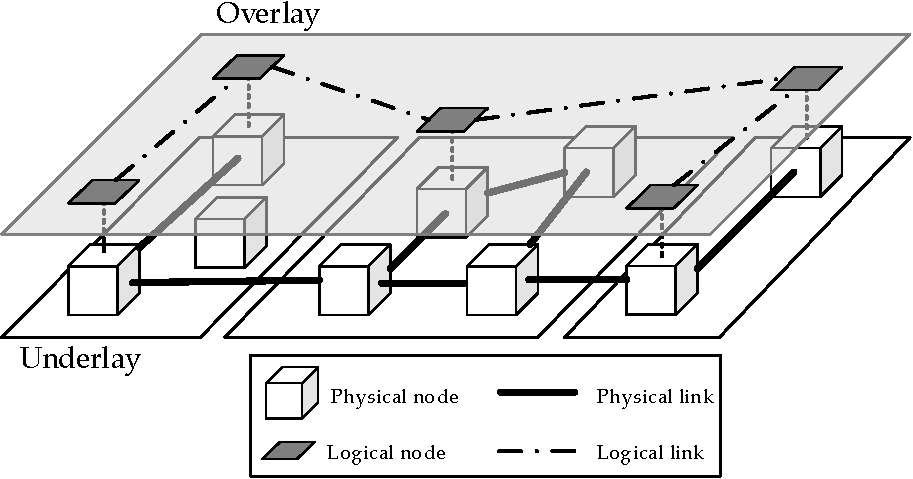
\includegraphics[width=0.65\textwidth]{figures/overlay.pdf}
  \caption[Overlay networking concept]{An overlay network on top of a physical underlay network which consists of three sub-networks}\label{fig:overlay}
\end{figure}

A distinction between two types of overlay networks is made: \emph{structured} and \emph{unstructured} ones. In the former, peers are organized in a specific, deterministic manner, such that each node has its firm place and an immutable set of neighbors. Unstructured overlay networks, on the other hand, allow the topology to change dynamically. In order for this to work, each node maintains an ad-hoc list of neighbors that is to be updated continuously \cite{tanenbaum2017distributed}. In the context of this thesis, unstructured overlay networks are of particular interest due to the dynamic nature and the reliability characteristics of mobile systems.

\paragraph{Virtual Local Area Networks.}
There are a number of ways to realize logical network overlays. VXLAN\footnote{``Virtual eXtensible Local Area Network''} and NVGRE\footnote{``Network Virtualization using Generic Routing Encapsulation''} two common examples which implement overlays on network datagram level. The technology used in the context of this work builds on VXLAN \cite{rfc7348}, an encapsulation protocol based on the long-established Virtual LAN (VLAN). VLANs make it possible to segregate a physical network into several isolated, logical networks. Each of those logical networks is assigned an identifier, a so-called \emph{VLAN tag}. All packets sent within a VLAN network have their respective network's VLAN tag attached on them at data link level (layer 2 in the OSI\footnote{``Open Systems Interconnect''} model). Based on the packet's tag, the substrate infrastructure can make decisions on how, and where, to forward packets. This allows for the realization of broadcast domains: each broadcast originating from a given VLAN network will stay within that network, regardless of how many other virtual networks exist alongside. This helps to significantly reduce network traffic.

Since the time when VLAN was devised much in the technological landscape has changed. In particular, virtualization has made great strides with the advent of cloud computing and multi-tenancy systems. Nowadays, thousands of virtual nodes dispersed throughout different clouds and on-premise infrastructures need to be connected. With its limited support for only 4096 virtual networks, VLAN cannot meet these increased demands. Thus, VXLAN was devised as a way to deal with the changed requirements.
The most notable changes, compared to VLAN, is the support for up to 16 million virtual networks and the option to assign addresses to \emph{processes}, rather than \emph{devices}.
In contrast to VLAN, which is an intrinsic part of layer 2 protocol frames, VXLAN is an independent protocol which is placed on top of UDP connections (in the application layer). This is illustrated \Cref{fig:vxlan} in which the VXLAN protocol stack is depicted. VXLAN works by wrapping the original data packet sent from one application to the other in a VXLAN frame which is then placed inside a UDP frame. As a result of this, two sets of addresses exist: the logical (source and destination) MAC addresses embedded in the encapsulated packet, and the physical MAC addresses in the surrounding packet.
Consequently, two types of packet switching need to be performed: once on a logical level, and once on a physical level. While physical switching is still performed inside physical network switches, an additional, logical type of switching needs to be introduced. Open~vSwitch~\cite{pfaff2015design} is an example of a virtual, software-based switch that performs packet switching in the data plane (within the Linux kernel).
\begin{figure}[htpb]
  \centering
  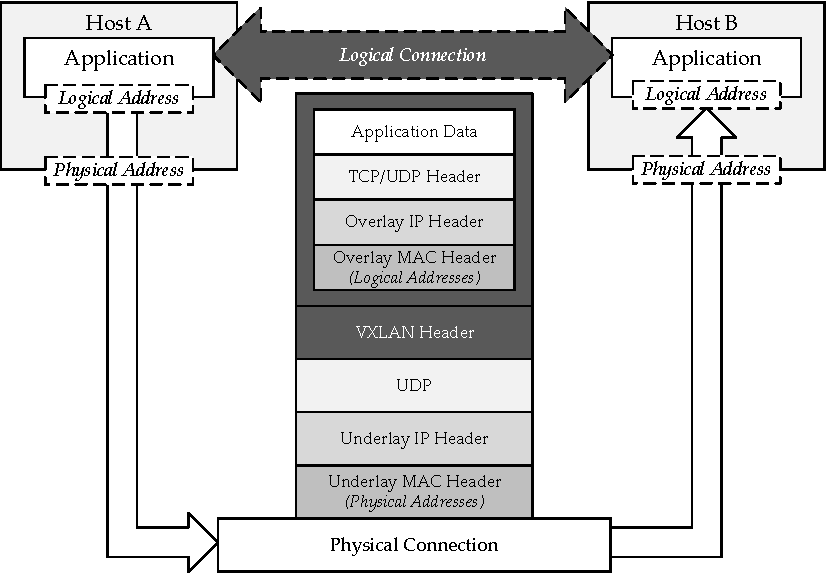
\includegraphics[width=0.6\textwidth]{figures/vxlan.pdf}
  \caption[VXLAN protocol stack]{VXLAN protocol stack exemplified by two logically connected applications}\label{fig:vxlan}
\end{figure}
Since VXLAN utilizes virtual MAC addresses that don't necessarily need to correspond to actual hardware addresses, addresses can be assigned at will for each process or virtual machine. This makes it possible to address single VM instances within an overlay network individually, regardless of physical locality and the underlying network design. An added benefit is that all endpoints may retain their logical address when migrating to other physical nodes. This allows for the creation of dynamically changing networks in which processes may move between different execution environments. Furthermore, VXLAN addresses the problem that WANs, in general, lack support for point-to-multipoint communication. In the context of an overlay network, peers may send messages to several receivers simultaneously, \eg\ by means of IP multicast, regardless of their physical location.
%Also included in the VXLAN header is a 24-bit network identifier which allows for the creation of 16 million virtual overlay networks, which is a tremendous step up from classic VLAN.

\pagebreak
In essence, VXLAN is a layer 2 overlay scheme on layer 3 networks which effectively creates \emph{tunnels} between Virtual Tunnel Endpoints (VTEPs), indicated by the dashed ``Logical Address'' boxes in \Cref{fig:vxlan}. Thus, logical connections in VXLAN overlays are often referred to as ``VXLAN tunnels''.
%Encapsulated within each VXLAN frame is the actual packet sent from one application to another. Addressing in VXLAN is based on MAC\footnote{``Media Access Control''} addresses.


%\subsection{Multicast}
%The simplest form of communication is one-to-one communication, which is also referred to as \emph{unicast}. In unicast, every node has an address by which it can be contacted. In most cases, unicast is sufficient for data exchange. However, in distributed systems, information frequently needs to be propagated to multiple receivers simultaneously. Unsurprisingly, this type of communication is called \emph{multicast} communication.

%benefits: No hard-coded addresses

%Multicast can be implemented on both, network and application-level.

%Support for multicast in WANs is rather limited.

\pagebreak
\section{Containerization}
In recent years, container technology has gained widespread adoption in the software development world. By providing light-weight, portable execution environments for applications, containers greatly simplify the software development and deployment workflow, and thus have become a cornerstone of modern software architectures.

\subsection{Comparison to Virtual Machines}
Containerization is also known as ``operating-system-level virtualization'' \cite{soltesz2007container}, and thereby disassociates itself from traditional virtualization technologies such as virtual machines. A major difference between the two is that containerization does not rely on an intermediate virtualization layer between application and hardware, whereas VMs employ hypervisors for this purpose. Hypervisors make it possible to run entire operating systems in their own, isolated environments, so-called VM instances. Several instances may run on the same host machine side-by-side without affecting one another, which allows for the realization of multi-tenant systems. Since hypervisors abstract the substrate hardware, a layer of indirection between hardware and the application to be executed is added. The consequence of this is a considerable overhead, compared to native execution. Containers, in contrast, run directly on the host's kernel and thus exhibit near-native performance (\cite{adufu2015container, felter2015updated, morabito2015hypervisors}). This approach, however, bears security issues~\cite{xavier2013performance}.

As mentioned, each VM instance contains its own operating system and kernel. As a consequence, the disk space requirements for VMs are comparatively high. Additionally, the guest OS within a VM needs to be booted into before being operational, which slows down the VM's start-up speed. Containers, in contrast, do not include their own OSes and kernels. Thus, container start-up can be performed in a matter of milliseconds and is more akin to spawning a process, rather than booting an OS. This enables them to be created and destroyed depending on situational demand, which allows for the implementation of highly elastically scaling systems.
%The recently emerged Function as a Service (FaaS) paradigm popularized by Amazon's cloud offering, AWS Lambda\footnote{\url{aws.amazon.com/de/lambda}}, even suggests to run an ephemeral container for each \emph{request}
Considering their advantages over hypervisor-based virtualization, such near-native performance, sub-second boot times, minimal disk space usage and their energy efficiency \cite{morabito2015power}, containers bring qualities to the table that are relevant especially to embedded systems, which are, by their very nature, resource-constrained. Unsurprisingly, the possibility of leveraging containerization in embedded environments has received substantial attention in recent years (\eg\  \cite{bellavista2017feasibility, javed2016container, morabito2017virtualization}).

Containerization and virtual machines are often regarded as competing virtualization technologies. However, both are not mutually exclusive. In fact, most IaaS providers base their infrastructure on traditional VMs, which then, in turn, host container runtimes~\cite{dua2014virtualization}. Containers and VMs shall thus be seen as complementary, rather than competing, technologies.

\subsection{Container Internals}
Like virtual machines, containers aim to isolate processes from their environment. In the case of containers, isolation is achieved by a kernel feature called \emph{kernel namespaces}.\footnote{\url{www.man7.org/linux/man-pages/man7/namespaces.7.html}} Namespaces wrap global system resources, such as network devices and mount points, and present them to processes as if they were dedicated to them.
When a process runs in the context of a certain namespace, its access and view is limited to that namespace.
There are seven types of namespaces, each of which isolates a different aspect of the host system.
An example for this are \emph{process} namespaces which allow for the creation of alternative views on the process tree. For instance, consider a hypothetical process with PID 345. By assigning a process namespace to that process, it can be led to believe that it has the PID 1 and is the only process running on the system. Thus, the processes' view on other processes is restricted, and since a process can only access what it can see, isolation is achieved.
In a similar way, a processes' access to networks interfaces, the file system, user groups and other parts of the host system can be restricted.

In addition to providing isolation, containers employ resource management mechanisms which make it possible to allocate and limit the resources available to them. Resource management for containers is implemented by a kernel feature called \emph{control groups}, or \emph{cgroups}\footnote{\url{www.man7.org/linux/man-pages/man7/cgroups.7.html}} in short. Cgroups allow for the organization of processes in hierarchical groups. On these groups, resource constraints can be imposed (\eg\ CPU-time, access to devices, memory budget, etc.).
Through this mechanism, processes can be bundled together, effectively forming \emph{containerized process trees}, which can be restricted in what they can do and which resources they may take up. This opens up the possibility for container engines to exert fine-grained control over each processes' resource utilization and to further isolate processes from the rest of the system.

The two concepts (namespaces and cgroups) can be applied individually to any given process running on a Linux system. Only when combined together, such that processes are isolated through namespaces and restricted through cgroups, we speak of containers. In consideration of this, it becomes clear that a containerized process is not much different from a regular process. Rather, containers should be viewed as processes which are \emph{augmented} by these two concepts.

%Further separation can be achieved through SELinux and AppArmor.

While it is possible to create containers manually utilizing the aforementioned native kernel features, such undertaking is rather cumbersome. For this reason, several tools are being developed which aim to streamline the use of containers. A few notable examples are \emph{\docker},\footnote{\url{www.docker.com}} \emph{RKT},\footnote{\url{www.github.com/rkt/rkt}} \emph{CRI-O},\footnote{\url{www.cri-o.io}} \emph{Railcar}\footnote{\url{www.github.com/oracle/railcar}} and \emph{LXC}.\footnote{\url{www.linuxcontainers.org}} Among these,  \docker\ is undoubtedly the most prominent one, and arguably the first one to make Linux containers accessible for general use. As it is the most mature containerization solution, \docker\ was chosen for the approach presented in this thesis.







%
%
%
%
%
%
%
%
%
%

%\section{Software Architectures}
%\todo[inline]{
%Today, there is a tendency for software architectures to shift away from the \emph{monolithic} paradigm of having a single software entity deployed on a single, potent server to a more \emph{distributed} paradigm where multiple components are spread over a number of less potent physical hosts connected over a network.
%The benefits of this approach became evident in the early 2000's when a new type of software architecture utilizing this concept became popular: \emph{service-oriented architectures} (SOAs).

%In recent years, SOAs have made a revival in the form of \emph{microservices}, which, in essence, is a more fine grained type of SOA that avoids the complexity induced by \emph{Enterprise-Service-Buses} (ESBs). Similar to SOA, the idea behind microservices is to split functionality into a collection of reusable components, each fulfilling a single specific purpose. Recent research efforts are evaluating the possibility to include such paradigm in the realm of automotive software systems -- in part achieving great success \cite{berger2017containerized}.

%Since Microservices are very limited in scope they may be built and deployed in a matter of minutes, rather than hours, as is the case with monolithic applications. Thus, microservices have the potential to tremendously accelerate the software development process when being combined with modern development practices such as \emph{continuous integration / continous delivery} (CI/CD).
%}


\chapter{Approach}\label{chapter:approach}

In this chapter, the main approach of this thesis is presented. The chapter starts with an abstract description of the approach with the aim of providing a high-level overview of the underlying concepts. Then, exemplary use cases are described, and finally, a list of requirements and desirable quality attributes is given (\autoref{sec:requirements}) which forms the basis for the evaluation part in \autoref{chapter:discussion}. 

%
%
%
%
%
%
%
%
%
%

\section{Concept} \label{sec:concept}
The objective of this thesis is to explore a new method to handle the increased demand for computational power and data collection in mobile cyber-physical systems, and in particular, automotive systems. For this, an approach is presented that allows for the outsourcing of vehicular functions to the cloud.
A special requirement is the unreliable connectivity common to mobile systems. To deal with this, the solution must be able to perform the offloading in an instantaneous, fail-safe, and automated fashion. When cloud connectivity cannot be provided, the operation of the vehicle mustn't be affected in any way and the previous state must be reestablished as soon as connectivity is restored.

%the cohesion of the system must be preserved at all times. 

\subsection{Partitioning of Functionality}
At the core of the approach is the idea to split functionality into isolated units which may be deployed redundantly on both, the vehicle's on-board system, and on high-performance machines in remote data centers. For this, the system needs to facilitate the clean separation of functionality according to responsibilities. The \emph{service-oriented} architectural paradigm \cite{erl2008soa} is a proven method for achieving this \todo{citation: generell SOA}. Service-orientated architectures aim to divide functionality into isolated, loosely coupled modules, so-called \emph{services}. Each service provides an offering to users, or other services, by means of a clearly defined, preferably immutable and machine-readable interface. By guaranteeing that these interfaces rarely change, a formal \emph{service contract} is put in place which ensures the continuous interoperability between the services. Examples of a service offering may be the provisioning of some sort of data, or functionality (algorithms and business logic) that is executed on behalf of a service consumer. All services of the system are working together like cogs in a machine to achieve a common goal, \ie , the continuous operation of a vehicle. 


\subsection{Communication}
Traditionally, E/E-architectures build on the principle of message buses as means to connect the system's dispersed components (ECUs)\todo{citation?}. In bus systems, all components write data samples to, and read data samples from, a shared medium (the bus). Individual components typically have no knowledge of each other's existence---they only know the data they provide and push it on the bus, or read the data they are interested in from the bus. This paradigm leads to a loosely coupled system in which components have as few dependencies among each other as possible. Loose coupling, in turn, tremendously facilitates extensibility and scalability. A concept closely related to message buses is the publish-subscribe principle by which service providers (publishers) and service consumers (subscribers) communicate on the basis of topics. In effect, a publish-subscribe system behaves in accordance with a bus system in which the shared medium is logically segregated into domains (\ie\ topics). 

In line with the traditional bus-centered nature of E/E-systems, the presented approach builds on a bus-like publish-subscribe paradigm. The characteristic that makes the envisaged bus special is that it virtually extends into the cloud. To facilitate this, a \emph{network overlay} \cite{tarkoma2010overlay} mechanism is needed. With the help of a virtual overlay network laid on top of the substrate network, a globally dispersed \emph{service mesh} may be created wherein the boundaries of the physical network lose their effect. That way, location-transparent messaging between services is achieved: it does not matter whether a given service runs within the vehicle or within the cloud---the way they communicate remains the same.

%\paragraph{}

%The last question that remains is how services are connected. Since services may be duplicated and migrated between computing nodes, special emphasis needs to be put on location/relocation transparency and dynamic topology management. In the approach, the use of virtual overlay networks is suggested for this purpose. Especially challenging is the fact that the overlay must work on top of a substrate network made up of numerous globally dispersed nodes, of which some continuously change their location. As a result, the substrate network is exceptionally unreliable.


%An inherent challenge distinctive to the domain at hand is the highly unreliable and unpredictable communication channel to the cloud. Remotely deployed services are thus ephemeral in their nature. As a consequence, the topology of the service network is constantly changing. This requires the communication method between services to be entirely anonymous. \Ie , services shall not have references to other services as these may be unavailable momentarily. Management of references (addition of new references and invalidation of old ones) is highly ineffective and therefore should be avoided at all costs. A communication paradigm that facilitates this is the publish-subscribe paradigm. In a publish-subscribe system, services exchange information by means of topics. Services that provide data may push data on a given topic, and services that wish to receive that data may subscribe to that topic. Services do not know where a given data sample came from or which service will receive their data sample. Thus, communication is anonymous.

%\todo[inline]{

%Switch must be feasible at run-time

%transition must be fluent

%Communication shall be ubiquitous

%A major problem in automotive architectures is the management of data. As a result of the historically grown nature, whereby each ECU is highly specialized in a very narrow range of duties, there is no consistent model of data---each ECU has its own view on data which may very well differ from other ECU's view \cite{broy2006challenges}. It is therefore evident that data need to be put into the center of attention. Data-centricity is a communication style that follows this goal. provides common, consistent view on data. global shared data space.
%}

%The method of exposition is data-centric: instead of providing \emph{methods} that other services may invoke (RPC style), services offer \emph{data}. Any service interested in receiving a certain kind of data listens in on a topic on which such data is published. This approach greatly helps to decouple the system as services do not need to have references to one another. As a result, services may evolve without having to deal with interface interdependencies.


\subsection{Replication}
The approach aims to achieve superior computing performance by way of horizontal scaling. Thus, replication is key. 
%Thus, the system shall support the fast provisioning of services in the form of \emph{service instances}. 
The service-oriented approach alleviates replication tremendously, provided that certain design principles are applied. Hence, throughout the design and implementation of the envisaged system, several design goals need to be kept in mind. Firstly, services ought to be \textbf{stateless}. Statelessness facilitates replication as sharing state among many instances proves to be difficult. Consistency within a distributed system is hard to achieve and locking mechanisms may introduce bottlenecks.\todo{more on consistency models this in tanenbaum...} A common practice to remove the need for such mechanisms is to avoid state altogether. 

Furthermore, services should be \textbf{fine-grained}. A high-resolution granularity allows for detailed control over which services should be replicated. That way, computational bottlenecks can be more easily singled-out and eliminated. An added benefit of fine granularity is an increase in extensibility and faster software updates. However, trade-offs need to be considered. If services are too fine-grained, they need to communicate more which may slow down the system. Furthermore, too many services unnecessarily increase complexity.

Another design goal to keep in mind is \textbf{isolation}. Services should have limited knowledge of other services' location and the system's topology. Through this, loose coupling is further promoted. One aspect of isolation is self-containment. Services should be bundled together with all their dependencies as a single unit that may be deployed on any hardware platform. By packaging services in self-contained environments, they may be moved between different computing nodes. This property is the most important one to achieve cloud scalability. Commonly used tools to facilitate this are virtualization and containerization.

\subsection{Example}
\begin{figure}[htpb]
  \centering
  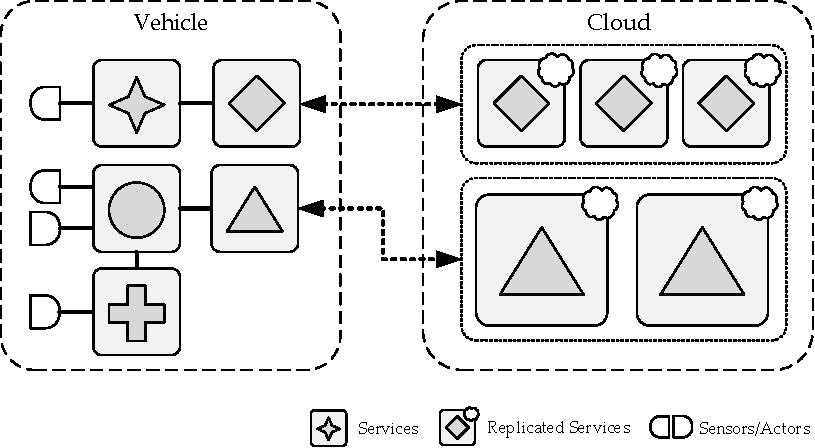
\includegraphics[width=0.9\textwidth]{figures/idea.pdf}
  \caption[Conceptual sketch of the approach]{Conceptual sketch of the approach}\label{fig:idea}
\end{figure}
\autoref{fig:idea} depicts a schematic example of the approach. The box on the left-hand side represents a vehicle. In the vehicle, several interconnected services are deployed. The figure omits any details regarding the actual computing infrastructure but only displays the general placement of services (either vehicle or cloud). In actuality, the the vehicular services run on distributed embedded devices spread over the vehicle's on-board system. Several of these services rely on sensor data and/or control actuators (indicated by the small semicircles). On the right-hand side, the cloud is depicted, which, in actuality, is a collection of high-performance computing nodes. Vehicle and cloud are physically separated and connected via some sort of network, which the vehicle may access by means of cellular networking technology. On a logical level, vehicular- and cloud-based services communicate via topics that may, or may not, span between the two otherwise isolated systems. Note that some of the vehicle-intrinsic services are replicated in the cloud (\ding{117}, \ding{115}). Examples of such services could be functions for calculating trajectories, computer vision-based gaze detection, or machine learning applications. The duplication and varying size of the service boxes depicted in the image is indicative of horizontal and vertical scaling, respectively. It doesn't always make sense to replicate services in the cloud, \eg , because they are computationally inexpensive, or because they require access to sensors and actuators which are inherently bound to the vehicle (\ding{70}, \ding{108}, \ding{58}). Those services have their firm place within the vehicle and are therefore referred to as \emph{fixed} services. Their counterpart, \ie , services that may run ubiquitously, are called \emph{volatile} services (\ding{117}, \ding{115}). A third kind of services are \emph{cloud-only} services, which are entirely optional and only serve to perform background tasks such as monitoring or persistence (\ding{86}, \ding{72}). Service \ding{72}, for example, would aggregate all data posted on Topic B and store it in a database. The discrepancy between fixed and volatile services emphasizes the need to split functionality into fine-grained services so that computational bottlenecks can be isolated and then eliminated. A good advice is to extract services connected to sensors and actuators in minimal ``access services'' (\ding{70}, \ding{108}, \ding{58}) that do nothing but provide access to sensor data.
%
%
%
%
%
%
%
%
%
%
\subsection{Key Challenges} 
\label{sec:challenges}
In the previous sections, a conceptual approach was presented to connect a vehicle's on-board system to the cloud to facilitate computation offloading, data collection, and other use cases. To achieve this, the approach suggests to split functionality into fine-grained services that may be replicated and migrated smoothly between vehicle and cloud. Three key challenges can be identified which need to be addressed in order to realize the system:

\begin{enumerate}[(i)]
\item \textbf{Reliable, anonymous information exchange}: Services must be able to communicate in a reliable manner, without the need for direct references to each other.
\item \textbf{Isolation}: Services need to be packaged in self-contained execution environments with all their dependencies to ensure portability.
\item \textbf{Connectivity}: Services need to be able to autonomously create and maintain connections between each other, regardless of their location.
\end{enumerate}
%
%
%
%
%
%
%
%
%
%
\section{Example Use Cases} \label{sec:usecases}
The presented system may be utilized in a number of ways. To further rationalize the system's usefulness it is helpful to keep a few usage scenarios in mind.

\paragraph{Supportive Autonomous Driving.}
A exemplary use case for the system is the offloading of computationally intensive functions to high performance computers in the cloud. 


Such functions are required, for instance, to facilitate autonomous driving. Especially machine learning- and computer vision algorithms often require high levels of parallelization. 
\todo[inline]{fertig schreiben}

\paragraph{Data Collection.} 
Another benefit of the approach is that it has the potential to greatly ease data collection. One could think of an example where passively listening services, implemented as subscribers, would run in the cloud at all times for the sole purpose of accumulating telematic/telemetry data. Due to the anonymous nature of the publish-subscribe paradigm, the vehicle's on-board system would be entirely oblivious of the listening services. The collected data could be used for real-time monitoring and analytics purposes, remote trouble shooting, or to feed machine learning algorithms running in the backend. Furthermore, location-based services and applications utilizing crowd-sourced traffic data would be possible. An example for this type of application is Google Maps' traffic congestion detection which is based on the accumulative GPS information collected from numerous user's Android phones.

\paragraph{Auxiliary Fail-Operational Behavior.}
The presented system allows services and their replicas to run side-by-side in the vehicle and the cloud. Multicast communication ensures that all service instances are always up-to-date\footnote{Provided that connectivity is given.}. It is now possible to realize fail-operational behavior by providing backup replicas of certain safety-critical services that would run in the cloud at all times. In the event that one of the vehicular services fails, \eg\ due to a hardware defect, the operation would not be interrupted as the cloud-based services would continue where the original service left off. If such case occurred in an autonomous driving scenario the vehicle would enter a temporary \emph{limp home} mode.
%
%
%
%
%
%
%
%
%
%
\section{Requirements and Quality Attributes} \label{sec:requirements}
The previous sections already touched on desirable quality attributes to keep in mind when implementing the approach. Still, a rigor requirement analysis is needed in order to be able to thoroughly evaluate it. To this end, a detailed requirement list is presented which an implementation of the envisaged system should aim to fulfill. The list is loosely based on the work of \citeauthor*{o2007quality} \cite{o2007quality}.

\todo[inline]{More info: Dependable systems [Kopetz, Verissimo]: Availability, Reliability, Safety, Maintainability}

\paragraph{Availability.}
Availability states how likely it is that, at any given point in time, a system is ready to be used by its users \cite{tanenbaum2017distributed}. The period in which a system or service is unavailable is called \emph{downtime}. Sources of downtime can be, \eg , maintenance work, temporary congestion, or any kind of failure. A design goal when building and running software systems is to minimize downtime, and thereby maximize availability. This goal is not trivial to achieve as many sources of decreased availability are hard to predict, \eg\ in case of hardware failures. A key technique for handling downtime is redundancy, whereby critical systems, or those susceptible to downtime, have a replacement ready to be used at all times. A prerequisite for redundancy to take effect is that the system features quick failure detection and smooth transition mechanisms so that it can quickly reroute requests to the redundant service. If a system manages to substitute an unavailable component in a way that is virtually unnoticeable, it is said to be failure transparent.

\paragraph{Reliability.}
Reliability states how long a system can continuously run without failure. A reliable system is available for prolonged periods of time without interruption. Although reliability is related to availability, there is a clear distinction between the two. While reliability concerns a continuous period of operability, availability is concerned with operability at a given point in time. For example, a system that works fine most of the time but becomes unavailable for a few milliseconds every hour is highly available, but not reliable. Hence, a highly reliable system is not necessarily a highly available one and vice versa \cite{tanenbaum2017distributed}. In real-time systems, a lack of reliability could easily result in the missing of deadlines, which in turn could have disastrous effects. In case of \emph{hard} real-time system, a single missed deadline is even equivalent to a complete system failure. Ensuring reliability is therefore of utmost importance. As with availability, a way to mitigate the effects of poor reliability is redundancy.

Special precautions need to be taken for \emph{distributed} systems as their communication channels are inherently unreliable \cite{tanenbaum2017distributed}. In practice, this means that the messaging system needs to provide guarantees for a timely and robust message delivery. In addition, certain assurances are desirable, \eg , that messages are delivered in order or that every message is delivered only once \cite{o2007quality}. 

\paragraph{Safety.}
The safety of system states how resilient \wrt\ failures it is, and in case a failure occurs, how well it can handle it. A safe system manages to protect the health and wellbeing of humans involved in the operation of the system and its surrounding bystanders.
As human lives are at stake in road traffic environments, vehicles are a prime example of systems that need to be safe.

Critical functions need to operate in a fail-operational fashion, \ie , in case they fail, the situation needs to be handled gracefully, without putting the passengers in danger. To this end, special precautions need to be taken throughout the whole process of development, provisioning, operation, and service of functions. ISO 26262 \cite{iso201126262} provides the standards that vehicular E/E systems need to adhere to in order to fulfill the necessary safety requirements. Different parts of the system need to be compliant to different classes of safety, indicated by automotive safety integrity levels (ASILs).

\paragraph{Security.}
In road traffic, flaws in a system's IT security have direct implications for safety. Since safety is of utmost importance the same is true for security. In today's world, vehicles are to a large extent software-driven \cite{broy2006challenges}. With an increasing number of lines of code comes an increase in complexity and error-proneness, and by that, a larger attack surface breaks open. Furthermore, vehicles are more and more connected to the outside world. Not only are they connected to third-party and OEM clouds, but also to other vehicles and the nearby infrastructure. The situation is made even worse by the fact that many of modern vehicle's subsystems can be controlled by software---even those which are safety critical.	 If an attacker were to gain access to, say, the steering system, consequences could be dire. Passengers would be put in severe danger.

To enhance security and to preserve the integrity, authenticity, and confidentiality of the system, state-of-the-art encryption and security measures are a necessity. To this end, proper isolation of software components is needed to build up security perimeters which are hard to penetrate. In case an attacker, or malicious code, succeeds in intruding the system, appropriate isolation measures, \ie\ sandboxing, can furthermore prevent the attacker from reaching out to other subsystems.

\paragraph{Interoperability.} 
In systems composed of a number of heterogeneous components that interact with each other, there needs to be a common set of rules and semantics that all involved parties must comply with. If such rules exist, so that diverse components may interact with each other, they are said to be interoperable.
A major barrier to interoperability is (vendor) lock-in. Lock-in describes a situation in which a certain technology is rooted so deep within the system that the introduction of alternative technologies can hardly be accomplished. Similarly, the technology is hard to remove without considerable effort. Lock-in is detrimental to system design as it creates dependencies, and thus, introduces tight coupling. Especially in the automotive domain, in which many parts of the system are developed by a vast number of independent teams and suppliers \cite{broy2006challenges}, interoperability should be a priority. Furthermore, OEMs tend to prefer a slow, stepwise transition towards innovative technologies, rather than jumping in at the deep end. Hence, automotive systems need to be particularly interoperable to existing solutions. A way to achieve a high degree of interoperability is to avoid proprietary, closed-source solutions and to favor open standards instead.

\paragraph{Performance.}
Performance is the amount of work that a computer system may accomplish within a given amount of time. A system may be performant in a number of ways. Common measures to gauge performance are, \eg , the time it takes to respond to a request (response time), the rate at which work is processed (throughput), or rate in which data is transmitted. Performance also states how efficient a system is in the utilization of hardware resources. This is important especially in embedded systems, where resource constraints are commonplace. Countless methods exist to improve a system's performance. One could make use of, \eg , concurrent programming models, compiled programming languages, or binary transmission protocols, to name a few. In the end, it is important to find an appropriate middle ground between performance and usability.

\paragraph{Scalability.}
Scalability is a system's ability to expand, or rather, deal with expansion. Often times, expansion is necessary to support an increased number of users or to deal with increased computational load. Generally, a distinction between two types of scalability is made: horizontal scalability, by which workload is distributed across an increased number of nodes (scaling out), and vertical scalability, by which a single node is upgraded with more powerful hardware (scaling up) \cite{tanenbaum2017distributed}. While vertical scalability is easier to realize, it is generally less desirable than horizontal scaling as there is an upper limit in how far it can scale. Furthermore, scaling up often involves downtime. Scaling out, on the other hand, is not affected by these shortcomings, and in addition to that, is in most cases more economical. However, horizontal scalability brings complexity, as many individual components need to be coordinated. Another challenge is posed by the question how load shall be distributed among the many components.

\paragraph{Extensibility.} 
Extensibility expresses how easy it is to add functionality to a system without affecting other parts of the system. This includes the extension of the system itself (by adding services), as well as the extension of individual services' functionality (by means of software updates) \cite{o2007quality}. The provisioning of new functionality must be possible not only at design-time but also at run-time. Modern automotive software architectures must deal with the fact that vehicular functions may be modified, added, or unlocked at run-time through (automatic) software updates. 
%At the same time, the preservation of service contracts must be a priority. Although formal service contracts are an absolute necessity, they may hinder innovation and the continuous evolution of the system. For this reason, the system must support the simultaneous operation of multiple versions of the same service side-by-side.

\paragraph{Adaptability.}
Adaptability is a measure for the amount of effort that is needed to change a system to accommodate for changes in requirements and the environment \cite{o2007quality}. Key properties of adaptable systems are autonomy, proper abstractions, and continuous monitoring\todo{why exactly?}. Adaptability needs to be addressed on many levels. Firstly, the system needs to be able to adapt to changes on software level. As a reaction to changes in the requirements, software needs to evolve. For this, software updates are inevitable, and thus, the system needs to accommodate for that. Another aspect of adaptability is concerned with the mobile nature of vehicles. Vehicles are connected to the outside world primarily by means of cellular networks. While moving, vehicles frequently change the access point, and hence, the topology changes continuously. The system must be able to reliably deal with changes in topology and exhibit great migration transparency properties. For this, service discovery must happen fully autonomously. 

Lastly, the system needs to be adaptable in terms of hardware. The goal is to run the same functionality in vehicles and the cloud side-by-side. For this, software needs to be portable between different hardware platforms. Different ways to address hardware interoperability exist. Common means to achieve a high degree of hardware adaptability are virtual machines, emulators and interpreted programming languages.


\paragraph{Testability.}
There are many ways in which a distributed system may break. Since operational safety is of paramount importance in the automotive domain, testability is a key requirement. Components of the system must be testable in isolation (\eg\ via unit tests) as well as in interplay with other components (\eg\ via integration tests). For this purpose, modern software development employs continuous integration tools that help to continually validate the correctness of a system throughout the whole development cycle. Automotive software architectures need to be adapted to make it feasible to employ such development practices.


%
%
%
%
%
%
%
%
%
%
\chapter{Realization} \label{chapter:realization}
After having discussed the basic concept of the approach in the previous chapter, in this chapter, an exemplary realization is presented. Previously, three key challenges were identified:
\begin{inparaenum}[(i)]
  \item \emph{reliable, anonymous information exchange},
  \item \emph{isolation}, and
  \item \emph{connectivity} (\cf \ref{sec:challenges}).
\end{inparaenum}
To tackle these challenges, three technologies are proposed:

\begin{enumerate}[(i)]
\item \textbf{DDS} to enable \emph{reliable, anonymous information exchange},
\item \textbf{\docker} as containerization tool to achieve \emph{isolation} and portability of services, and
\item \textbf{\wnet} as means to provide \emph{connectivity} between the containerized services.
\end{enumerate}

In the following, these three tools are presented and it is described how they are leveraged to realize the proof of concept implementation.


\section{Data Distribution Service for Data Exchange}
Data Distribution Service (DDS) is a messaging middleware standard \cite{dds-1.4-standard} for distributed applications governed by the Object Management Group (OMG).\footnote{\url{www.omg.org}} DDS is designed for mission- and business critical systems with real-time requirements. As such, it aims to function in a resource efficient, predictable and reliable manner, and is subject to minimal computational and transport overhead.
Thus, DDS is a great fit for the automotive use case. 

\subsection{Data-Centric Publish-Subscribe}
DDS is fundamentally based on the data-centric publish-subscribe (DCPS) communication paradigm. In the publish-subscribe-style communication, data flows between two kinds of entities: publishers and subscribers. Publishers provide data, while subscribers consume that data. A crucial characteristic of publish-subscribe is that data exchange between the peers is anonymous, \ie , publishers have no way of sending data to individual subscribers. Instead, both communicate by means of a shared, logical medium that takes data samples and forwards them to the appropriate receivers. In the context of DDS, this medium is called \emph{topic}. When subscribers receive a data sample they do not know where that sample originated. Similarly, publishers have no knowledge about where the sent data will end up at---or even if there are any receivers at all. Entities in this system find each other not by way of addressing, but rather on the basis of a shared understanding of what \emph{kind of data} they want to exchange. This approach is called \emph{data centricity}. Data centricity is in contrast to \emph{message centricity}, in which data exchange is driven by \emph{messages}, or \emph{instructions}, which are directed at individual receivers. A prominent example of a message-centric technology is Remote Procedure Call (RPC). To illustrate the difference between the two paradigms consider the example of a temperature sensor (henceforth also ``provider'') which propagates temperature data to multiple receivers (henceforth ``consumers'').

\paragraph{Message-Centric Approach.} In the message-centric paradigm, the temperature sensor transmits data samples encapsulated in \emph{messages} to the consumers. Messages are directed at each consumer individually, similar to a letter that is addressed to a certain postal address. This requires each participant to maintain their peers' location information (\ie\ their addresses) in local memory.
Two patterns are common in message-centric communication: ``push-based'', and ``pull-based'' (often ``request-reply''-style) communication~\cite{tanenbaum2017distributed}.

If message-centric communication is push-based, the sensor needs to know the addresses of all interested consumers a-priori. The provider thus has to maintain a list of consumers that it needs to update continuously. When a previously uninvolved consumer decides that it wants to receive temperature data, it first needs to register to the sensor in order to make its address known. The sensor then has to add the consumer's address to its list of consumers. Similarly, when a consumer is shut down, the sensor needs to remove the respective address, and has to deal with unexpected errors in case a consumer is suddenly unreachable. This (un)registration procedure is the cause of overhead and additional management effort, and makes the system inflexible and hard to scale. In contrast, pull-based communication don't rely on lists of consumers, but consumers request information from the provider. In this regard, pull-based communication is more scalable, however, additional overhead is incurred since two messages (instead of one) need to be transmitted for each data sample: a request and a response. Furthermore, consumers can not predict when a new data sample is available. The situation is made worse when there is not one producer, but many. Thus, both approaches are highly inefficient in the use case at hand.

\paragraph{Data-Centric Approach.} The DCPS approach, on the other hand, is exclusively push-based.\footnote{Although request-reply-style communication is not explicitly supported it can be mimicked (\cf \Cref{sec:ddslatency}).} The temperature sensor is a publisher in the publish-subscribe relationship, and the consumers are subscribers. A subscriber that is interested in the sensor's data only knows that it wants to receive \emph{temperature data}, \ie\ data samples of type ``temperature'', and thus, subscribes to the ``temperature'' topic. 
The temperature topic is defined by a unique identifier and a data type. Only data of that specific type may be published on the topic. To ease the use of the middleware, DDS provides typed interfaces to the exchanged data. Through the optional \emph{Data Local Reconstruction Layer} (DLRL) \cite{dlrl-1.4-standard}, data types can be defined via the DDS IDL,\footnote{``Interface Description Language''} and according language-specific stubs can be generated. The use of type safe interfaces not only improves usability, but also increases safety and error-proneness, as verifications can be performed at compile time.

In the temperature sensor example, the subscriber is entirely oblivious to the concept of \emph{temperature sensors}, or even if there are any sensors---it just listens in on the ``temperature'' topic. Similarly, the temperature sensor is only concerned with the provisioning of temperature data, and doesn't know which subscribers to send the data to. Thus, the temperature sensor publishes all samples it gathers on the ``temperature'' topic. If more temperature sensors were to be introduced to the system, they could simply be added by registering new publishers which would post data on the same topic. Since all publishers of a topic identify themselves purely on the basis of their topic, and not by their address or location, a great deal of redundancy can be achieved---all publishers of a given topic are entirely interchangeable.
Due to the agnostic relationship between publishers and subscribers, a high level of loose coupling is achieved. This allows for a simple extension of the system, making it extraordinarily scalable.

It is often helpful to think of publish-subscribe communication not in terms of messages that are sent from one entity to another, but rather as a \emph{shared global data space} in which data is universally accessible to all entities involved in the system. In this data space, each entity views data as if it were available in a local storage, when in reality, it is distributed among many other entities.

\subsection{Under the Hood}
Naturally, in order to realize a publish-subscribe system, addresses and locations of nodes are still crucial, as publish-subscribe, like other communication paradigms, rely on IP-based computer networks. This fact, however, is hidden behind the curtains of the middleware (DDS in this case). The middleware is responsible for the registration of publishers/subscribers, the dissemination of data to the appropriate receivers, and the enforcement of network reliability policies. In order to do this efficiently, the middleware maintains lists of subscribers, publishers and topics. Many middlewares employ central components called ``brokers'' for this. Depending on the view point and use case, the centralized nature of brokers may be considered advantageous, or disadvantageous. On the one hand, centralization is associated with simplicity since everything is managed in one spot, and only one single source of truth exists. On the other hand, this approach brings the danger of a single point of failure that causes the whole system to fail if the broker fails. Additionally, centralized brokers may introduce bottlenecks, inhibiting the scalability of the system. 
As DDS is strongly focused on scalability, DDS employs a \emph{brokerless} architecture in which the functionality of the communication system is distributed among all participating entities. Consequently, message delivery as well as service discovery is performed in a decentralized manner.
For this, DDS may optionally employ IP multicast, by which all communication is directed at dedicated multicast group addresses, instead of each node's individual address. The delivery of data is then the responsibility of the underlying infrastructure.

\subsection{Wire Protocol}
DDS, in itself, is only a standard. As such, DDS does not dictate, in detail, how to implement the concepts presented in the earlier sections. A number of DDS implementations from different vendors exist, all varying in terms of standard compliance, features beyond the standard, licensing, and other distinguishing factors. Compatibility between the respective implementations can be achieved by the use of the DDSI-RTPS\footnote{The ``DDSI'' in DDSI-RTPS is often omitted. The shortened form will henceforth be used.} (DDS Interoperability--Real-Time Publish-Subscribe) wire protocol, which all major implementations support. Although the RTPS protocol is directly related to DDS, its specifics are outsourced in a separate standard \cite{rtps-2.2-standard}.
As a wire protocol, RTPS is deliberately tailored to DCPS-style communication. As such, it supports reliable multicast-enabled data exchange and service discovery over unreliable and connectionless best-effort transports such as UDP/IP. Special emphasis is put on robustness, fault tolerance, scalability and performance. Thus, RTPS was conceptualized with safety-critical real-time applications in mind. Although RTPS is the preferred transport method for DDS applications, it is not the only option. Many DDS vendors support TCP, UDP, and shared memory for cases in which performance is critical.

%
%
%
%
%
%
%
%
%
%
%
%
%
%
\subsection{DDS Components}
The DDS specification defines a number of components which are introduced in the following. \Cref{fig:dds} depicts an example highlighting how the components are related. In the example, there are two hardware nodes connected by an unspecified computer network. Each node can execute multiple applications simultaneously. The applications communicate with each other by means of DDS.


\begin{figure}[htpb]
  \centering
  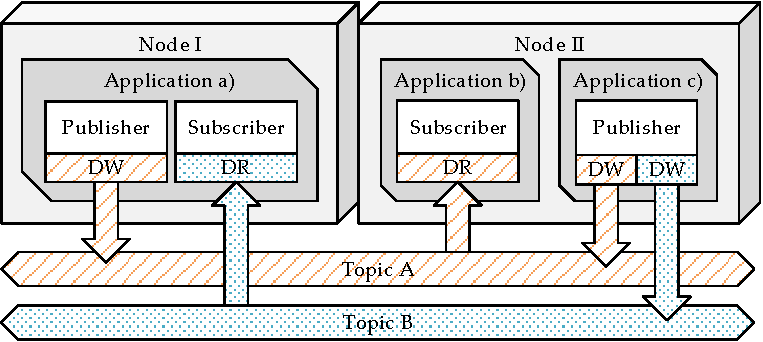
\includegraphics[width=0.8\textwidth]{figures/dds.pdf}
  \caption[An example of a distributed application connected via DDS]{An example of a distributed application connected via DDS}\label{fig:dds}
\end{figure}

\paragraph{Topics.}
\emph{Topics} form the basis on which peers communicate in the publish-subscribe paradigm. When a Publisher offers a certain kind of data, it does so by means of a Topic. When a data sample should be written, the Publisher pushes that data sample to a Topic appropriate for that sort of data. Conversely, when a Subscriber is interested in receiving data of a certain kind, then it subscribes to a Topic associated with that data. A Topic is uniquely defined by an identifier (name), a data type, and a set of QoS policies (see below). The data type represents the message format for data samples published on that Topic. For example, a suitable data type for a Topic concerned with temperature data would be a \texttt{struct} containing a single \texttt{float} value representing a temperature reading.
In \Cref{fig:dds} two Topics are depicted (Topic A and Topic B), each with a number of associated Data Writers and Data Readers (see below).

\paragraph{Publishers and Data Writers.}
\emph{Publishers} are entities that provide information in the publish-subscribe communication paradigm. Publishers are not bound to a single Topic. Instead, they contain one or more \emph{Data Writers}, each dedicated to a single Topic, who perform the actual data submission. Thus, Publishers may be seen as containers for a number of (unrelated) Data Writers. This concept is emphasized in \Cref{fig:dds} where a Publisher in Application c) controls two independent Data Writers that both write to different Topics.

\paragraph{Subscribers and Data Readers.}
\emph{Subscribers} are the exact compliment to Publishers in that they seek to receive data from Publishers. Analogous to Publishers, Subscribers are a way to group together sets of \emph{Data Readers}. Data Readers are entities whose purpose it is to receive data samples from their respective Topic. Through its API, DDS allows Data Writers to receive data in three ways: either by waiting for data samples (blocking the main thread), by pro-actively polling for new data samples, or by specifying asynchronous callbacks which are invoked whenever a data sample arrives.

\paragraph{Domains and Domain Participants.}
\emph{Domains} are the DDS way of grouping together sets of coherent \emph{Domain Participants} and to separate those sets from each other. Speaking in terms of distributed systems, Domains are a mechanism to manage group memberships of nodes \cite{tanenbaum2017distributed}. Domain Participants are entities that belong to a particular Domain. Each Publisher, Subscriber and Topic is derived from one Domain Participant and is therefore dedicated to exactly that Domain. As a consequence, participants of different Domains are entirely separated from each other and there is no way for them to interface with each other. Depicted in \Cref{fig:dds} is only one Domain. However, there could just as well be other Domains.
\pagebreak
\subsection{Quality of Service}
One of DDS's salient features is its intrinsic support for Quality of Service (QoS), which is realized by so-called ``QoS policies''. QoS policies specify attributes that can be used to control each component's behavior and quality properties. They make specifying a component's behavior a matter of \emph{configuration}, rather than \emph{implementation}. For example, consider a Data Writer which writes data to a Topic at a high rate. A Data Reader may be interested in that data but not at such a high rate, \eg\ because it runs on an embedded device powered by a battery and therefore needs to manage power consumption carefully. The Data Reader may now apply a \tbf , which instructs DDS to block all samples that exceed a specified frequency threshold. This way, the rate of incoming messages can be controlled via configuration. This is beneficial for the programmer as they do not need to accommodate for this at code level, but let the middleware take care of it.

QoS policies can be set for each Topic, Publisher, Subscriber, Data Writer and Data Reader individually.
In \Cref{tab:qos}, an excerpt of the available QoS policies is given. For the exhaustive list of all available QoS policies refer to the official standard \cite{dds-1.4-standard}.

Another example of a QoS policy is the \deadline\ policy. It specifies the minimum sampling frequency of a Data Writer. If the deadline period of a hypothetical Data Writer is set to, e.g., 100 ms, then this Data Writer is obligated to send a data sample at least every 100 ms. If it fails to send samples at this rate, the Data Writer and all the respective Topic's readers will be notified about that circumstance and are free to act accordingly.

In addition to specifying quality attributes, QoS policies may also serve as ``service contracts'' between interacting DDS components. These contracts specify non-functional requirements that the involved components must fulfill to be able to communicate with each other. For example, a Data Writer's \reliability\ policy may have been set to the \texttt{BEST\_EFFORT} level, thereby allowing the writer to drop samples. A Data Reader, on the other hand, may require the writer's policy to be set to \texttt{RELIABLE}, which prohibits the dropping of samples. Since the writer does not fulfill the reader's QoS requirements, the two components are considered incompatible, and thus, they cannot interact with each other.

Despite their name, QoS policies do not only concern \emph{quality} attributes per se. They can also be used to specify the priority of data samples, their lifespan, \ie , how long they are valid, or how many data samples of a certain type are kept in local memory.


\begin{table}[H]
  \caption[An excerpt of DDS QoS policies]{An excerpt of QoS policies}\label{tab:qos}
  \centering
  \begin{tabular}{p{0.25\textwidth} p{0.2\textwidth}  p{0.45\textwidth}}
    \toprule
      \textbf{Name} & \textbf{Legal values} & \textbf{Description} \\
    \midrule
    	\reliability  & \texttt{RELIABLE}, \texttt{BEST\_EFFORT} & Indicates whether a Data Writer may drop samples or whether a Data Reader approves of Data Writers that drop samples.\\
    	\tbf  & An integer value denoting time & Specifies a Data Reader's desired data reception rate. Superfluous samples will be discarded.\\
    	\liveliness  & An integer value denoting time & Defines the rules to determine whether a particular entity is ``alive'', \eg\ by emitting heart beats. \\
    	\deadline  & An integer value denoting time & Establishes a contract between Data Writer and Data Reader to determine the acceptable data rate. \\
    	\ownership  & \texttt{SHARED}, \texttt{EXCLUSIVE} & Specifies whether multiple Data Writers may write to a given Topic simultaneously or just the one with the highest \ostrength\  value.\\
    	\ostrength  & An integer value denoting relative priority & Determines a Data Writer's priority in cases where its Topic's \ownership\ is set to \texttt{EXCLUSIVE}. \\
    \bottomrule
  \end{tabular}
\end{table}
%
%
%
%
%
%
%
%
%
%
%
%
\pagebreak
\subsection{Redundancy and Automatic Failover} \label{sec:failover}
DDS has ways to ensure reliable communication---even over unreliable transmission channels. Part of reliability is failure transparency, \ie , the ability to quickly substitute failed components by backup components. The substitution process involves two steps: first, the failure needs to be detected. Second, a backup component needs to be instructed to take over. By means of the three QoS policies \ownership , \ostrength\ and \liveliness\ (\cf \Cref{tab:qos}), DDS may realize this process.

As the first step, a mechanism needs to determine whether a component has failed. In most cases, it is not possible for a failing component to properly shut down and ``sign off'', \ie , to notify the rest of the system that it will become unavailable. For this reason, the failure needs to be automatically registered. The \liveliness\ policy can be used to achieve this. \liveliness\ is the mechanism that determines whether a component is responsive (``alive''), or unresponsive (``dead''). The policy's value can be set to number indicating the maximum time interval between each liveliness signal. If a component fails to show a vital sign during that period, it is considered dead by the rest of the system. Passive components, \ie\ those which do not actively emit data, can be instructed to automatically send liveliness signals, or heartbeats, in certain intervals.

After a component has been declared dead it is up to the middleware to elect a substitute component. This is done through the \ownership\ and \ostrength\ QoS policies. By assigning a topic the \ownership\ value ``\qos{exclusive}'' one can specify that only a single data writer may write to that topic at any given time. Which data writer is given that prerogative is determined by the data writer's \ostrength\ value. The data writer that possesses the higher value is eligible to write to the topic. In the failover scenario, both, the primary data writer and the backup writer are assigned to the same topic, and both are configured to have exclusive \ownership\ rights. The former one has a higher \ostrength\ than the latter one. Based on both writer's \ostrength\ values, it is decided which one has precedence over the other.
%
%
%
%
%
%
%
%
%
%
%
%
%\subsection{Separation of User Data}
%The presented approach relies on a single cloud infrastructure, while at the same time, a vast number of customers need to be served. This poses a challenge concerning the separation of data. Confidentiality and privacy of user-specific application data must be preserved. Similarly, the result of a computation commissioned by a specific vehicle must be returned to exactly that vehicle, and no one else.

%Gladly, DDS offers a solution to this. In DDS, topics are not restricted to a single domain, \ie , they may be reused in multiple domains. If, \eg , a publisher belongs to \texttt{Domain $\alpha$} and publishes data on \texttt{Topic A}. Then, a data reader that reads from \texttt{Topic A} but belongs to \texttt{Domain $\beta$} may not read the data. Therefore, through domains, the same application may be reused several times on the same network, while keeping topic data separate. This principle is taken advantage of in the presented approach: domains are used to separate user data, such that for each user there is one user-specific domain. Thus, there is no way that data from one vehicle may interfere with data from another vehicle.

%\subsection{DDS for Automotive Systems}
%Automotive software systems have previously relied---and, to some degree, will continue to do so---on low-level, low-bandwidth transport protocols such as CAN, LIN, etc. For the longest time, networks stacks based on those protocols were sufficient to meet the basic requirements of delivering vehicular sensor data. However, driven by the emergence of innovative functions, the demands for vehicle intrinsic networks are skyrocketing. In particular, more and more sensor data from increasingly bandwidth-hungry sensors, such as cameras and lidars is feeding into advanced systems such as ADAS.
%At the same time, these functions require computational capabilities that go way beyond of what is possible with the microcontrollers typically used in traditional ECUs. High-performance computer systems based on high-level operating systems, supported by bandwidth-friendly networking protocols are needed to meet the new requirements.
%A new generation of low-level network protocols found their way into the vehicle. Notable mentions are FlexRay, and TSN. A question that remains is whether DDS is a suitable choice for the use within vehicles, and whether DDS may be used efficiently on top of these lower level protocols. \citeauthor*{bouhouch2013dds} have shown \cite{bouhouch2013dds} that DDS is indeed a suitable middleware to be used in vehicular networks.

%DDS allows to configure how much of a system's resources an DDS-enabled application may use. Consequently, it is the middleware's responsibility to allocate resources as needed while still staying within the specified boundaries. At the same time, priorities aligning with the application's QoS settings need to be considered. DDS takes this burden off the programmer's shoulders.
%\todo[inline]{TODO}


%
%
%
%
%
%
%
%
%
%
%
%
%
%
%
%
%
%
%
%


%
%
%
%
%
%
%
%
%
%
\pagebreak
\section{\docker\ for Containerization}
In this thesis' approach, services and their dependencies shall be encapsulated in their own, self-contained execution environments that may be deployed inside the vehicle and also in the cloud. Containerization is a promising technology to achieve this. For the exemplary implementation, \docker\ is used as it provides an easy-to-use interface and is available for x86, as well as for ARM-based platforms.

\docker\ is a holistic containerization platform which includes everything needed to build, run, deploy, and distribute containers. The \docker\ application is structured in a client-server model (\cf \Cref{fig:docker-arch}). The server is a daemon process running at all times on the host machine. Its primary purpose is to manage containers, images, networks and data volumes, and to provide the means to  build images and run containers. The \docker\ server exposes a RESTful HTTP API by which it can be controlled. The client side of the \docker\ application is a command line interface (CLI) which acts as a user friendly façade for the server's API.\footnote{\url{docs.docker.com/engine/docker-overview}}

\begin{figure}[htpb]
  \centering
  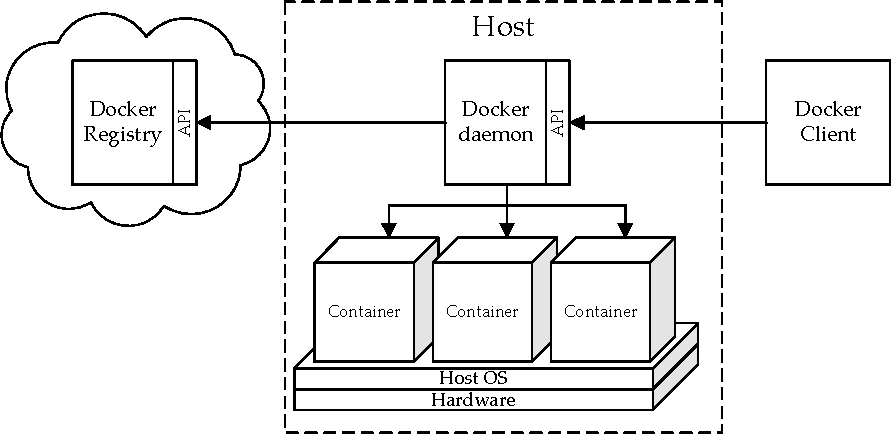
\includegraphics[width=0.7\textwidth]{figures/docker-arch.pdf}
  \caption[\docker\ architecture]{\docker\ architecture}\label{fig:docker-arch}
\end{figure}

\pagebreak
\subsection{\docker\ Components}
\paragraph{\docker\ Images.}
Images are a central component of \docker . They may be seen as the ``blueprint'' on the basis of which containers are built and define exactly which files and directories are contained in a container once it comes to life. Effectively, every container is an instantiation of an image of a certain type, in the same way an object is an instantiation of a class in an object-oriented programming language. While the concept of images is very common among containerization and virtualization tools, \docker\ follows a rather unconventional approach.
In \docker , images are made up of series of read-only file system layers stacked on top of each other. Each layer may add files and directories to its respective underlying layer. If a layer tries to modify a file from an underlying layer it creates a copy of that file and adds it to its own layer. The modification is then performed on the copy instead of the original. This principle called ``Copy on Write'' (CoW) ensures that layers cannot be modified which makes it possible to share individual layers with other images stored on the host. An example of this is later described in \Cref{sec:containerized-services}. By treating images as a collection of individual, sharable pieces instead of atomic units, massive storage space savings can be achieved. Another benefit of this is that whenever a container is started, only a thin writable layer needs to be added on top of an image, and the underlying layers do not need to be copied. That way, start-up times of containers are kept extremely low.\footnote{\url{docs.docker.com/storage/storagedriver}} Virtual Machines, in contrast, would first need to boot into an operating system prior to operation.

\paragraph{Dockerfiles.}
\docker\ images are defined in so-called Dockerfiles.\footnote{\url{docs.docker.com/engine/reference/builder}} Dockerfiles are made up of series of instructions that tell \docker\ how to build a certain image. Each instruction adds another file system layer to the image.
\begin{lstlisting}[caption=An examplary Dockerfile, label=lst:dockerfile, numbers=left, numberstyle=\tiny]
FROM debian
COPY . /application
RUN cd /application && make
ENTRYPOINT /application/run.sh
\end{lstlisting}
An example of a Dockerfile is depicted in \Cref{lst:dockerfile}. The first line of this Dockerfile defines the base image on top of which this particular image shall be built. In this case, an image called ``debian'' was chosen. As the name suggests, that base image contains a basic installation of the Linux distribution Debian.\footnote{\url{www.debian.org}} Next, the line \ \mbox{\texttt{COPY . /application}} \ instructs \docker\ to copy the contents of the current (host) directory to the container's \ \mbox{\texttt{/application}} \ directory. Due to \docker 's CoW approach, the changes in the file system are added in the form of a layer---the underlying layers are not affected. The \ \texttt{RUN} \ instruction in the following line causes \docker\ to run the subsequent commands within the container. In this case, the newly added application directory is entered and the command \ \texttt{make} \ is executed, effectively compiling the application. Again, the resulting changes to the file system are encapsulated within another layer. In practice, the now topmost layer would contain all files produced by \ \texttt{make}. Finally, the \ \mbox{\texttt{ENTRYPOINT}} \ instruction defines the action to be performed once the container is started. In this case, the shell script \ \texttt{run.sh} \ would be executed within the container. This command, too, would add a layer to the image, albeit an empty one. By defining images as sequences of instructions, reproducibility is guaranteed.
By running the command \ \mbox{\texttt{docker build -t IMAGENAME .}} \ in the directory of the Dockerfile, an image based on that Dockerfile would be built. Using the command \ \mbox{\texttt{docker run IMAGENAME}}, a new container of that image type would be launched.

\paragraph{\docker\ Registries.}
\docker\ images may be stored in \docker\ Registries,\footnote{\url{docs.docker.com/registry}} where they can be browsed, managed, and distributed. The command \linebreak \texttt{docker push IMAGENAME[:TAG]} \ causes the image with the name \ \mbox{\texttt{IMAGENAME}} \ to be uploaded to a registry. Analogously, to download an image from a registry to the local computer, one would have to run the command \ \mbox{\texttt{docker pull IMAGENAME[:TAG]}}. \docker\ registries are implemented as a server software which exposes an HTTP API (\cf \Cref{fig:docker-arch}). The registry server is open source\footnote{\url{www.github.com/docker/distribution}} and may be deployed on any server that supports it. The \docker\ company itself hosts one of such registries, Docker Hub,\footnote{\url{hub.docker.com}} which is provided as a publicly available  and free-to-use service.
\pagebreak
\subsection{Multi-Platform Compatibility} \label{sec:multiplat}
The primary purpose of containerization is to provide portable execution environments that allow software to run on a broad range of computing systems. A limitation of containers is that they only provide portability across \emph{operating systems}, and not \emph{hardware platforms}. In other words, containers do not provide binary compatibility. The reason for this is that containerized applications run directly on the kernel of the host system, and do not build on top of a virtualization layer as classic VMs do. As a result, a containerized binary built for an x86-based processor will not run on an ARM system, and vice versa. This is problematic especially in the context of embedded systems which often rely on particular hardware architectures that favor energy efficiency over performance. Computing nodes in a data centers, on the other hand, are typically based on architectures aimed at providing a maximum level of performance. As the presented approach intends containers to be deployed on both, vehicular on-board systems and in the cloud, this poses a challenge. Two approaches exist to tackle this problem.

\subsubsection{Universal, QEMU-enabled Images}
The first approach relies on a thin platform compatibility layer that is put into the base of each container. This approach was popularized by resin.io, a company that specializes in containerization for IoT devices. On their Docker Hub page\footnote{\url{hub.docker.com/u/resin}} they provide \docker\ images which have the QEMU\footnote{\url{www.qemu.org}} machine emulator built in. Facilitated by QEMU's user emulation mode, binaries built for a given processor architecture may be executed on otherwise incompatible processors. QEMU achieves this by translating any guest system calls into host system calls. The previously mentioned images are built in a way that allows any arbitrary binary executed within such container to be run in the context of QEMU. Thus, the container may run on a multitude of hardware platforms.
This approach simplifies the software build process tremendously as only one universal container per service needs to be built. This container can then be reused for all platforms.

\pagebreak
\subsubsection{Manifest Lookup}

The QEMU approach has a significant drawback: multicast is not well supported by QEMU, which is why the idea was discarded.
Thus, another approach was leveraged to solve the multi-platform compatibility issue. This approach builds on Continuous Integration (CI) in accord with Docker Hub, and in particular, Docker Hub's \emph{image manifest} feature. The concept of image manifests builds on the following premise: by default, a \docker\ image name corresponds to exactly \emph{one} image. Thus, whenever an image with a given name is requested from the \docker\ registry, only that specific image is returned to the requester. Image manifests extend registries by the option to define \emph{multiple} images per image name. That way, several containers, each specifically built for a given platform, may be deployed under the same name. Depending on the requesting node's hardware architecture, a different image may be returned. \Cref{fig:manifest-pull} depicts an example for this. In the example, an x86-based machine requests the \ \mbox{\texttt{some/image:v1.0}} \ image from the registry. What is then returned from the registry is an image specifically made for x86 architectures. On the other hand, an ARM-based machine which requests the very same image, \ \mbox{\texttt{some/image:v1.0}}, receives an entirely different image as a response. This kind of behavior is achieved through an image lookup in the manifest file which is performed behind the scenes.

\begin{figure}[htpb]
  \centering
  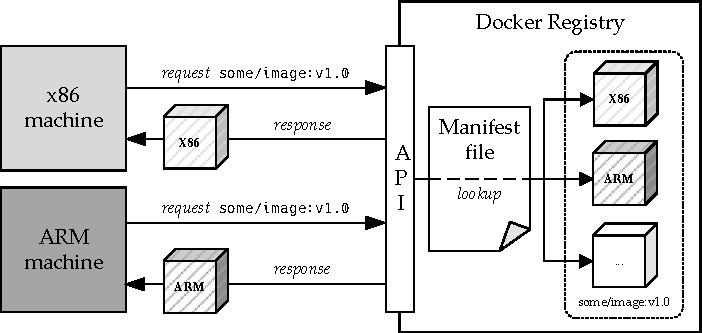
\includegraphics[width=0.6\textwidth]{figures/manifest-pull}
  \caption[Pulling \docker\ images via manifest file]{Two nodes request the same image name but receive different images which are specifically built for their respective processor architecture. Which node requires which image is determined by a look-up in the manifest file.}\label{fig:manifest-pull}
\end{figure}

\begin{figure}[htpb]
  \centering
  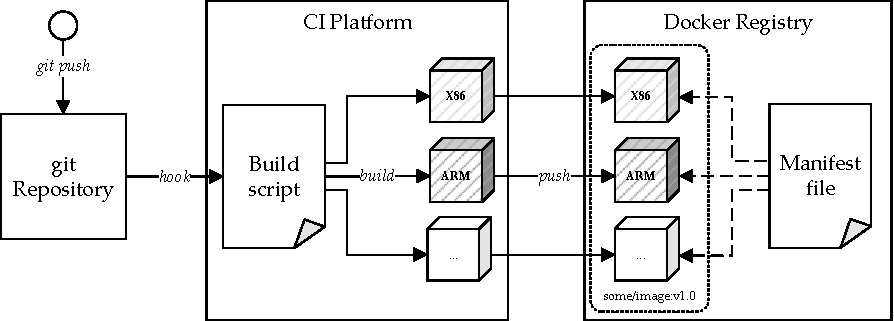
\includegraphics[width=0.7\textwidth]{figures/manifest-push}
  \caption[Pushing \docker\ images via CI]{A git push to a service's git repository triggers the build process in the CI platform: the code is compiled for several platforms and the resulting images are pushed to the \docker\ registry.}\label{fig:manifest-push}
\end{figure}

A disadvantage of this approach (compared to the QEMU one) is that multiple versions of the same container need to be built every time a service receives a software update. To cope with this hindrance, a minimal CI pipeline was leveraged. Consider \Cref{fig:manifest-push} in which the employed service deployment process is depicted. The build process is initiated whenever a code change is pushed to the remote git repository. Once a push is registered, the CI Platform (Travis CI\footnote{\url{www.travis-ci.org}} was used) pulls the latest version from the git repository and executes a build script. The build script compiles several version of the service for each target platform, embeds the binaries in images and pushes those images to the \docker\ registry (Docker Hub). Thus, several images, each tailored to a different platform, may be built and deployed in one go.


%
%
%
%
%
%
%
%
%
%
%
\subsection{Containerized Services} \label{sec:containerized-services}
In the envisaged system, each service is packed into its own container with all its dependencies. That way, services may run wherever they are placed, and thus, a great deal of portability is achieved.

\Cref{fig:service-containers} shows an example of three containerized services running on two different machines, \experim{Host I} and \experim{Host II}. On the former, two instances of \experim{Service A}, and one instance of \experim{Service B} are placed. On the second host only one service instance is deployed, namely one of type \experim{Service C}. All services are packaged in their own, separate container. The containers are made up of three stacked images---the bottom two are common to all services. The bottommost image (``\emph{base image}'') contains the file system layers of a minimal operating system. In this thesis, the Linux distribution Debian was used. The base image only contains a limited selection of Linux tools, such as \ \texttt{ls}, \texttt{cat}, \texttt{ps} \ etc. The purpose of a base image is to lay a solid foundation that enables users to work comfortably within the container. In the case of Debian, the \emph{aptitude} package manager is additionally included which enables users to easily install further tools.

Next, an \emph{intermediate image} is built on top of the base image. The intermediate image adds further layers containing the services' run-time environment, and in particular, the shared libraries of OpenDDS. This image could optionally contain additional libraries and tools that are common to all services. For the purpose of demonstration, however, DDS on its own is sufficient. The base image and the intermediate image lay the foundation of all services. Any image built on top of these could run any DDS-enabled application. Facilitated by \docker 's layered approach to images, the bottom two images can be shared among all services deployed on a host. In the example, the base image and the intermediate image both only need to be stored once on \experim{Host I}, which saves tremendous amounts of disk space.

\begin{figure}[htpb]
  \centering
  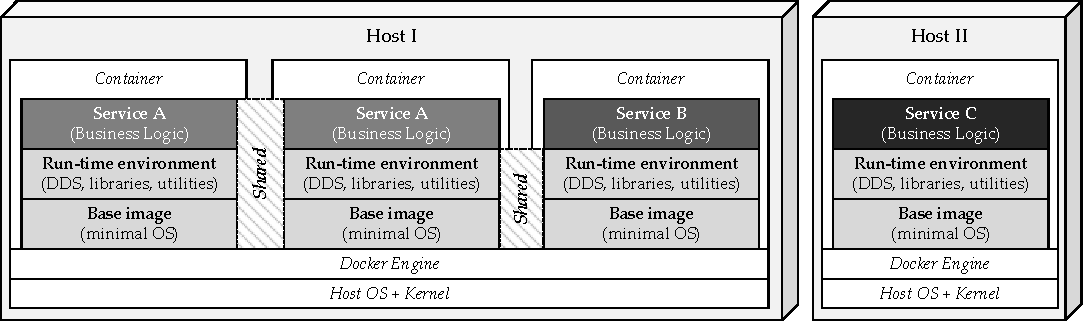
\includegraphics[width=\textwidth]{figures/docker-sharing}
  \caption[An example of containerized services]{An example of four containerized service instances, some sharing common logic to save disk space and facilitate fast updates}\label{fig:service-containers}
\end{figure}

At the top, finally, sit the \emph{service images}. In these images contained is the actual service logic, and more precisely, the service's binary and configuration files. The service images are unique to each service, and are not shared, except when the same service is instantiated multiple times on the same machine (\cf \experim{Service A} in \Cref{fig:service-containers}).



\section{Container Networking with \wnet}
\wnet\ is an open source project\footnote{\url{www.github.com/weaveworks/weave}} which is developed by a global team, mostly employed by the London-based software company \emph{Weaveworks}\footnote{\url{www.weave.works}}. The purpose of \wnet\ is to provide advanced overlay networking capabilities for \docker\ containers. As such, is designed to make up for the shortcomings of \docker 's built-in overlay networks, and more specifically, their lack of encryption and multicast support. By means of \weave\ overlay networks, dispersed containers deployed on physically isolated hosts around the world, may communicate as if they were connected via LAN. From a containerized applications' viewpoint, it does not matter whether its peers are located on the same host or within a data center on the other side of the world. 

\paragraph{}

\wnet\ is implemented as client software which is installed on each machine that partakes in the overlay. The software can be started using a single command, and in the following, all containers launched on that host will automatically connected to the overlay network. This is achieved by means of a \emph{\docker\ API proxy}. The proxy sits between \docker 's command-line client and the \docker\ daemon and intercepts all communication between the two. When the \docker\ engine is instructed to start a container, the proxy takes all precautions needed to enable overlay networking for that container. Once the connection is established, all container traffic is routed through three dedicated network channels: one TCP connection to exchange meta data about the network, and two UDP channels for duplex data exchange.

\begin{figure}[htpb]
  \centering
  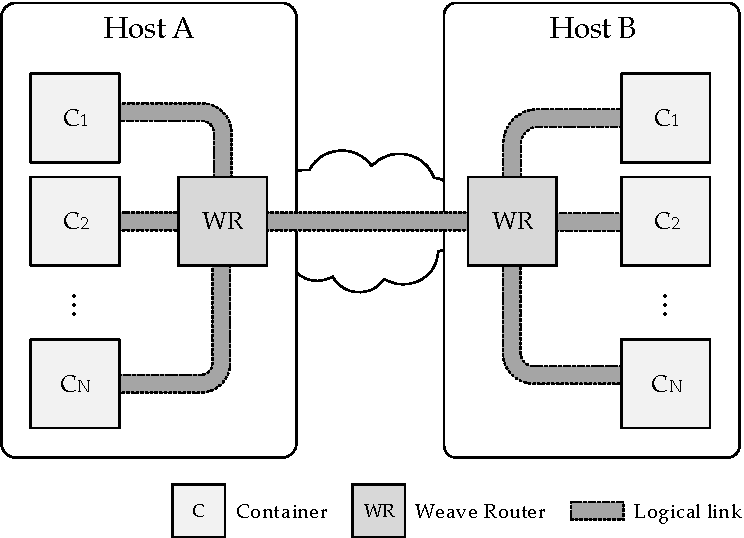
\includegraphics[width=0.7\textwidth]{figures/weave.pdf}
  \caption[An example of containers connected via \wnet\ overlay network]{A number of dispersed containers connected by a \wnet\ overlay network}\label{fig:weavescheme} 
\end{figure}

When the \weave\ software is started, a central component of \wnet , the \emph{\weave\ router} is launched (\cf\ \autoref{fig:weavescheme}). Similar to a hardware router, the \weave\ router is responsible for the forwarding and routing of data packets to their appropriate receivers. \weave\ routers can be seen as gateways through which all containers participating in a \weave\ network are connected. To facilitate routing on the data plane, a custom UDP encapsulation protocol, called \emph{sleeve}, was devised. A \weave\ router in itself is an containerized application running at all times, in the same way a daemon would. There is one of such router containers running on every host in a \weave -enabled infrastructure.

\todo[inline]{ÜBERARBEITEN}

The \weave\ router is a user space process. As such, a context switch is needed every time it is tasked to process a packet. This comes with a substantial performance overhead. Hence, as a faster alternative, the so-called \emph{fast datapath} mode was added. In this mode, packets are processed by the Linux kernel instead of by the \weave\ router. This way, the context switch into user space is omitted. \wnet\ leverages the Linux kernel's \emph{Open vSwitch datapath} module \cite{pfaff2015design} to achieve this behavior. Open vSwitch can be used to create a virtual, software-based network switch. That way, the kernel can be instructed to process packets in a certain way. For instance, the kernel can be commanded to add a VXLAN header to each packet, thereby achieving the same result as the \weave\ router, but faster. However, fast datapath mode can only be used when the underlying infrastructure allows it. The Internet is a particular example of a network where fast datapath communication is hard to achieve.


\subsection{Topology Management} 
\weave 's topology management is self-governing and self-healing. Peers continually exchange topology information and monitor the state of the network. Whenever peers lose connectivity, they continuously try to re-establish the connection until it is restored. All participating peers know the topology of the entire network. For this, \wnet\ employs a sophisticated discovery and topology management mechanism by which changes in the network topology are rapidly propagated within the network. The topology management protocol is based on a spanning-tree broadcast mechanism known from hardware switches. To further ensure that all peers have an up-to-date neighbor list at all times, \wnet\ additionally employs a custom neighbor gossiping protocol by which each peer sends update messages to a random subset of their neighbors. Updates of the network's topology are performed periodically as well as when certain events occur, such as when a node joins or leaves the network.

In order to add a new host to the overlay, the \weave\ software needs to be started on that host, referencing at least one other host in the network by its IP address. The information that a new host was added is then propagated to the other hosts in the overlay. After a short period, all hosts know that the new host was added and that a path to that host exists.

\subsection{Encryption} 
As mentioned earlier, a salient feature of \wnet\ is the ability to encrypt all traffic within the overlay network\footnote{Encryption applies end-to-end between \weave\ routers}. This is especially important for networks that span over insecure underlays, such as the Internet. To set up encryption, a shared secret (password) needs to be provided when the \weave\ router is launched. The shared secret must therefore be present on all participating hosts. From the password, salted, ephemeral session keys are generated which are then used to encrypt the network packets' payload. For each connection between any two peers, one unique session key exists.

The way encryption is applied differs depending on the forwarding mode used (sleeve or fast datapath). In fast datapath mode, a IPsec-based protocol is used, whereby each packet is wrapped in an encapsulated security payload (ESP). Because each packet in this mode is processed by the Linux kernel, encryption is applied by means of the standard Linux Kernel Crypto API which is thoroughly tested, and generally considered secure. For sleeve mode, a custom encryption algorithm based on TLS\footnote{``Transport Layer Security''} is used. As with fast datapath encryption, sleeve mode encryption utilizes shared, ephemeral session keys for each connection.

\begin{figure}[htpb]
  \centering
  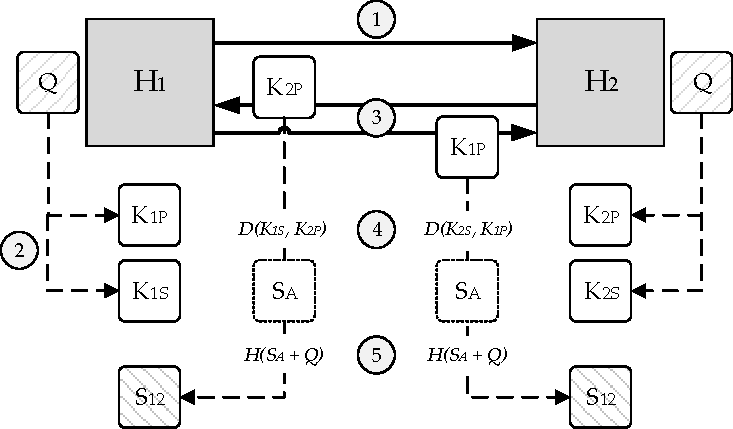
\includegraphics[width=0.6\textwidth]{figures/weave-encryption.pdf}
  \caption[\weave 's key exchange protocol]{\wnet 's key exchange protocol in sleeve mode}\label{fig:weaveencryption}
\end{figure} 
\autoref{fig:weaveencryption} depicts how these session keys are generated. In the image, two hosts ($H_1$, $H_2$) are to establish an encrypted connection. First, $H_1$ initiates the key exchange by sending a handshake message to $H_2$ \circled{1}. Then, both hosts generate their own, individual key pairs so that each host has a public key and a private key \circled{2}. The key pair for $H_1$ is $(K_{1P}, K_{1S})$ and the key pair for $H_2$ is $(K_{2P}, K_{2S})$. Once that is done, both hosts exchange their respective public keys, $K_{1P}$, and $K_{2P}$ \circled{3}. Using the peer's public key and their own private key, both hosts derive an auxiliary shared key, $S_A$, by means of Diffie--Hellman key exchange \cite{bresson2001provably}: $D(K_{1S},K_{2P})$ \circled{4}. Finally, the actual shared key can be generated. For this, both hosts append the password ($P$) to $S_A$ to provide authenticity. In order to bring the key to the desired length of 256 bit, the compounded key is additionally hashed via SHA256: $H(S_A, P)$ \circled{5}. The end result of this procedure is the final shared key, $S_{12}$, which is then used to encrypt the traffic between the two hosts.
%
%
%
%
%
%
%
%
%
%
%
%
%
%
%
%
%
%
%
%










\chapter{Evaluation}\label{chapter:evaluation}

In the previous chapter this thesis' main approach was presented and an exemplary implementation based on well-established technologies was suggested. What now follows is an evaluation of the implementation. Points of interest are the system's performance characteristics, reliability properties and general feasibility. For the purpose of evaluation a number of tests were conducted which are presented in the following. But first, the experiment setup is thoroughly described.


\section{Experimental Setup}\label{sec:testsetup}

As part of the \emph{Osborne} \todo{ist das richtig? link?} project a testbed was developed...
\todo[inline]{finish introduction}

The network topology used in the tests is depicted in \autoref{fig:network-topology}. In the local test environment ("on-premise") there was a cluster of three ARM-based SOCs\footnote{System on a Chip} (Raspberry Pi 3) whose network interfaces were connected by a Gigabit LAN switch (left-hand side). The three nodes represent on-board computing devices in a hypothetical vehicle. Connected to the LAN was also a workstation which fulfilled the sole purpose of orchestrating the tests, \ie , it was not directly involved in the test execution per se. The local test environment was connected to the remote data center over the open Internet via 100 Mbit/s connection.

\begin{figure}[htpb]
  \centering
  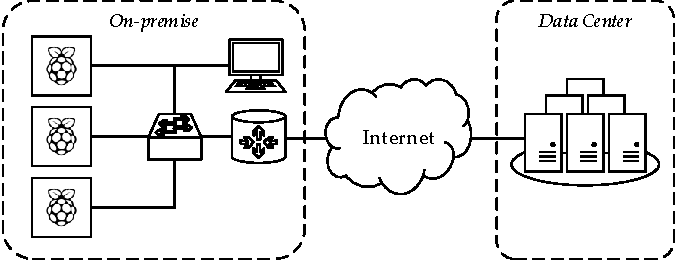
\includegraphics[width=\textwidth]{figures/network-setup}
  \caption[Network topology of the experimental setup]{The experimental setup's network topology}\label{fig:network-topology}\todo[inline]{copy rights on raspberry pi logo?}
\end{figure}
%
Representative of the "cloud" in the tests is a single root server supplied by the IaaS provider \emph{DigitalOcean}\footnote{\url{www.digitalocean.com}} (right-hand side in \autoref{fig:network-topology}). To ensure realistic latency values, a server location was chosen that was in the vicinity of the test setup -- but not too close. Considering its vicinity to Munich, Frankfurt (Main) was a suitable choice. The two cities are about 300 km away from each other (as the crow flies).

Throughout the whole study the software composition remained unchanged. As DDS implementation \emph{OpenDDS}\footnote{\url{www.opendds.org}} was chosen. The middleware was configured to utilize dynamic service discovery (no service repository) and RTPS over UDP as wire protocol. The optional Data Local Reconstruction Layer (DLRL) was used, by which messages are converted into type safe data structures. This causes some overhead which was evaluated and discussed in \autoref{sec:ddslatency}. Generally, default QoS settings were used for the tests, except in cases where a point was made to explicitly deviate from the defaults, \eg , the \liveliness\ settings in \autoref{sec:failovertest}. Moreover, all benchmarks were programmed in C++ to maximize their run time performance.

Naturally, in the benchmarks concerned with the testing of \wnet  , containers were connected by means of a \wnet\ overlay network. For the connection between all local nodes (on-premise), fast datapath forwarding mode was used. Due to the characteristics of the network between the local nodes and the cloud, fast datapath was not applicable for that connection. Consequently, local containers and cloud containers were connected via sleeve mode.

The detailed specifications of the involved computing nodes and the employed software are given in \autoref{tab:test-specs}
%
\begin{table}[htpb]
  \caption[Test environment specifications]{Test environment specifications}\label{tab:test-specs}\todo[inline]{check again}
  \centering
  \begin{tabular}{p{0.235\textwidth} | p{0.335\textwidth}  p{0.335\textwidth}}
    \toprule
       & \textbf{On-premise} & \textbf{Remote} \\
    \midrule
    	Description & Raspberry Pi 3 Model B  & DigitalOcean 1 GB Droplet\\
    	Number of nodes & 3  & 1\\
      Network connection  & 100 Mbit/s & 40 Gbit/s\\
    	\midrule
    	Operating system & Raspbian GNU/Linux 9.3  & Ubuntu 16.04.3 LTS\\
    	Kernel & 4.9.59-v7+ w/ real-time patch \emph{PREEMPT\_RT} 4.4.9-rt17 & 4.4.0-112-generic \\
      CPU & ARMv7 rev 5  Quad Core (1.2 GHz) & Intel(R) Xeon(R) E5-2650 v4 Single Core (2.20GHz) x86\_64 \\
      Memory (RAM) & 1 GB & 1 GB  \\
      Network interface  & 100 Mbit/s & ?? Gbit/s\\
      \midrule
      DDS & \multicolumn{2}{c}{OpenDDS 3.12.1}\\
      Docker  & \multicolumn{2}{c}{17.11.6-ce}\\
      \wnet & \multicolumn{2}{c}{2.2.0}\\
    \bottomrule
  \end{tabular}
\end{table}
%
%
%
%
%
%
%
%
%
%

\section{Benchmarks}

\subsection{Latency Benchmark} \label{sec:plainlatency}

\paragraph{Motivation.} An essential non-functional requirement for computer networks is responsiveness. An often-used metric for responsiveness is latency which is measured by the time it takes for a packet to be sent from one peer to another and back again. The unit of this measure is round-trip time (RTT), which is typically indicated in milliseconds. 

To evaluate the aptitude of the proposed approach it is essential to consider the latency overhead that overlay networks induce. Since the approach is intended to work over the Internet, and public networks are inherently insecure, encryption is vital. Thus, in addition to the overhead induced by the overlay network itself, the overhead caused by encryption is also of interest. Hence, tests are needed measuring latency not only of \emph{plain} overlay networks but also of \emph{encrypted} overlay networks.


\paragraph{Methodology.} 

\begin{figure}[htpb]
  \centering
  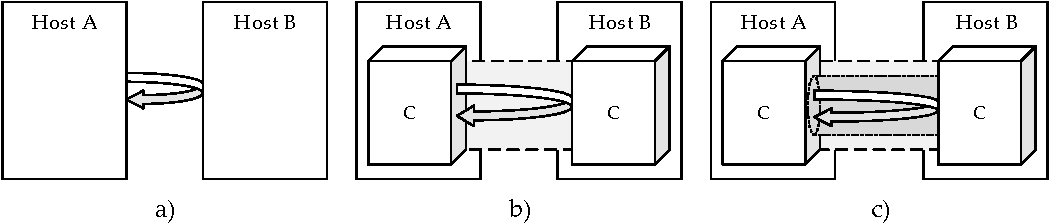
\includegraphics[width=\textwidth]{figures/ping-test}
  \caption[Latency experiment setup]{Latency experiment setup. a) \experim{Plain}: two hosts connected without overlay network. b) \experim{Weave}: two containers connected via \wnet . c) \experim{Encrypted}: two containers connected via encrypted \wnet\ .}\label{fig:latency-setup}
\end{figure}

In this test, latency was measured between two hosts connected over the Internet, both with, and without overlay-enabled container networking. A constant stream of ping messages was sent from one of the Raspberry Pis to the remote host. The tests were repeated with multiple payload sizes to factor in the influence of message size on round trip times. The Linux tool \emph{ping}, which pings hosts via ICMP Echo Requests and Replies, was employed for the measurements. 

Three experiments were conducted, comparing the average latencies of plain, host-to-host communication ("\experim{Plain}"), via \wnet\ ("\experim{Weave}") and when employing encryption over \wnet\ ("\experim{Encrypted}") (\cf \autoref{fig:latency-setup}). \experim{Plain} was used as baseline on the basis of which the two consecutive experiments were evaluated. For each experiment and message size, 300 ping messages were sent. The sending peer would wait for the response of the previous message before sending another request. Thus, only one transaction was in flight at a time.


\paragraph{Results.} 
\autoref{fig:latency-relative} depicts the absolute and relative latency measures of the tested network modes. Values represent the average round trip time of the 300 sent messages. The relative overhead is calculated from ratio of \experim{Weave} and \experim{Encrypted} when compared to \experim{Plain}, respectively. The results show that the network latency induced by \wnet\ (without encryption) is hardly measurable and therefore negligible. Message size has no influence whatsoever in this comparison. 


\begin{figure}[htpb]
  \centering
  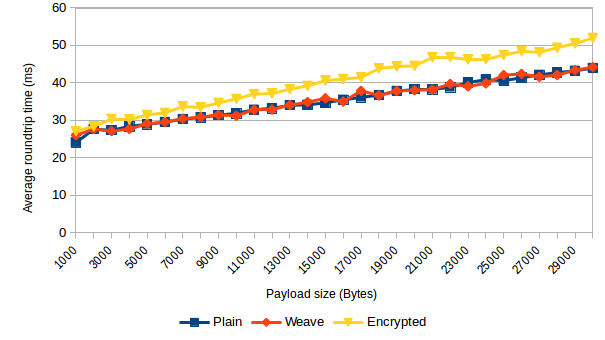
\includegraphics[width=0.49\textwidth]{figures/latency-absolute}
  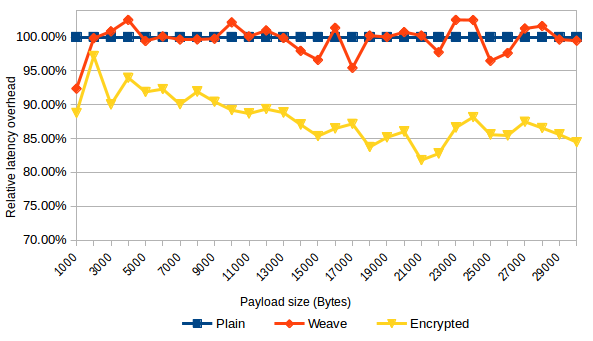
\includegraphics[width=0.49\textwidth]{figures/latency-relative}
  \caption[Latency overhead]{Absolute (a) and relative (b) latency overhead of \experim{Weave} and \experim{Encrypted} over \experim{Plain}}\label{fig:latency-relative}
\end{figure}

However, the tests revealed that encryption over \wnet\ (\experim{Encrypted}) adds quite a hefty base overhead which further increases with message size. For the smallest messages the overhead started at roughly 5\% and went up to over 15\% for messages with 30 KB payload. The encryption overhead may therefore be considered significant.

\begin{figure}[htpb]
  \centering
  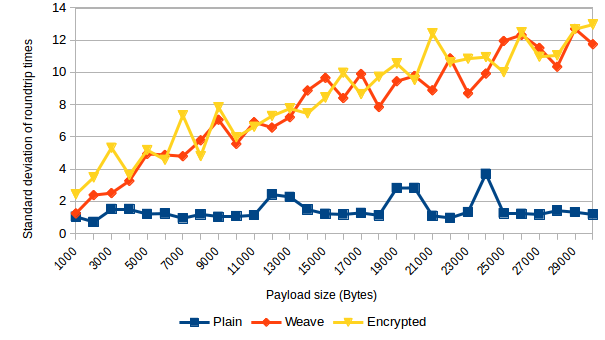
\includegraphics[width=0.8\textwidth]{figures/latency-stdev}
  \caption[Latency deviation]{Standard deviation of latencies in the scenarios \experim{Plain}, \experim{Weave} and \experim{Encrypted}}\label{fig:latency-stdev}
\end{figure}

Another insight worth mentioning is that \wnet\ added significant deviations in latency that increased with message size (\cf \autoref{fig:latency-stdev}). Whether the connection was encrypted or not made little difference. Real-time systems need to behave in a predictable manner. The experiments show that routing traffic through overlay networks had a substantial, negative impact on predictability of the communication channel. From the viewpoint of real-time systems this is a serious drawback of the presented approach. 



%
%
%
%
%
%
%
%
%
%

\subsection{Throughput Benchmark} \label{sec:throughput}

\paragraph{Motivation.} Another important metric for network performance is throughput. Throughput is a measure for how much data can be transmitted per time. Since little data is available on \wnet 's throughput performance, according tests were conducted.

\paragraph{Methodology.} To measure throughput, the tool \emph{iperf3}\footnote{\url{www.iperf.fr}} was used. iperf continuously sends data from one node to another over a TCP/IP connection. From the volume of the transmitted data and the duration of the transmission, the effective network throughput can be calculated. iperf was set to transmit data for a relatively long time period of 60 seconds to produce meaningful results. As in the previous test, three scenarios were tested:  \experim{Plain}, \experim{Weave}, and \experim{Encryped}. Explanations of these scenarios can be found in the description of the previous test.

\paragraph{Results.} The results of this benchmark are depicted in \autoref{fig:throughput}. The results show that unencrypted \wnet\ adds a minor throughput overhead when compared to \experim{Plain} scenario (5\%). When adding encryption to the overlay network, a minor additional overhead can be observed. Overall, encryption incurs an overhead of 6.7\% compared to \experim{Plain}. These values can be considered decent. 


\begin{figure}[htpb]
  \centering
  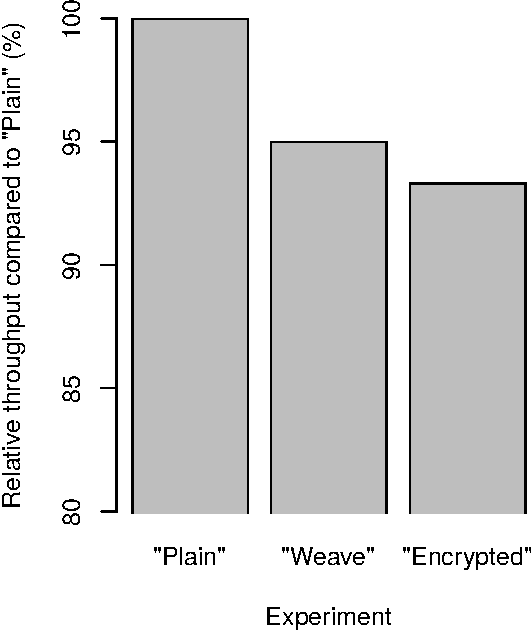
\includegraphics[width=0.8\textwidth]{figures/throughput}
  \caption[Weave throughput benchmark results]{Relative throughput in the scenarios \experim{Plain}, \experim{Weave} and \experim{Encrypted}}\label{fig:throughput}
\end{figure}

%
%
%
%
%
%
%
%
%
%


\subsection{Resource Utilization Test} \label{sec:utilization}

\paragraph{Motivation.} The routing of data packets through an overlay puts significant load on the host's CPU. Under circumstances, the forwarding of data, which is typically an IO-bound operation, might become CPU-bound, \ie , the CPU becomes the bottleneck of the operation. In cyber-physical systems, in which computing resources are limited, this might be problematic. Hence, an experiment was designed aimed to evaluate the impact of overlays on CPU utilization.

\paragraph{Methodology.} In this experiment, sample data was sent from a Raspberry Pi to the remote host via iperf (\cf \autoref{sec:throughput}) over an encrypted \wnet\ overlay. During the time of data transmission, CPU utilization was measured using the Linux tool \emph{sar}. 25 test runs were conducted using different bandwidth settings: bandwidth was gradually increased in 1 Mbit/s increments, starting at 1 Mbit/s, and ending in 25 Mbit/s. This bandwidth will be called \emph{target bandwidth} in the following. The target bandwidth is succumbed to an artificially imposed limitation and may differ quite substantially from the bandwidth that is actually achieved. The achieved bandwidth will be called \emph{observed bandwidth}, or \emph{throughput}.

\paragraph{Results.} 

\begin{figure}[htpb]
  \centering
  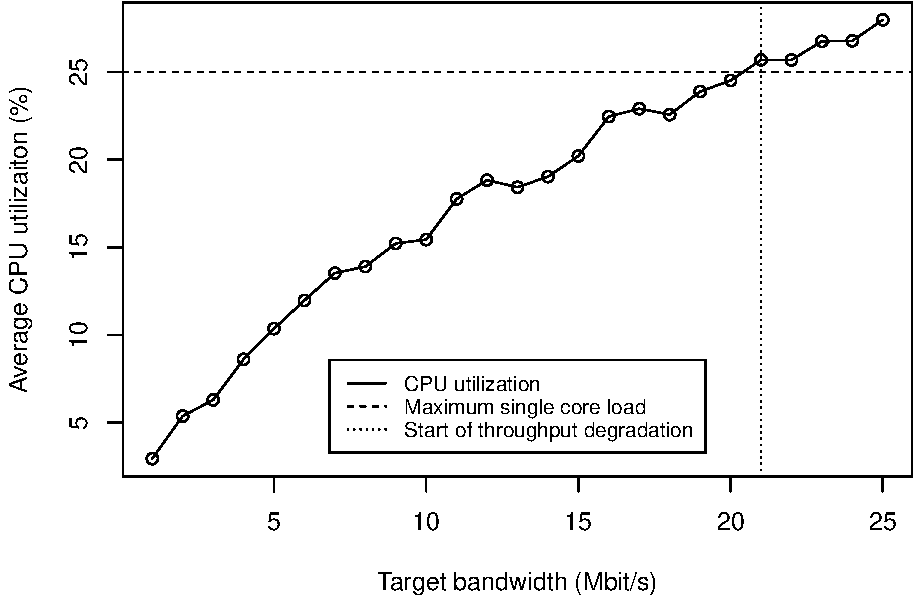
\includegraphics[width=0.8\textwidth]{figures/cpu}
  \caption[Weave CPU utilization test results]{Bandwidth and CPU utilization}\label{fig:cpu}
\end{figure}

\autoref{fig:cpu} depicts the test results. In the diagram, each data sample represents the average CPU utilization during a test run. The Y-axis represents the overall CPU utilization of the "sending" machine (Raspberry Pi), and includes the cumulative load of all programs running on the system. Hence, the measurements include a bit of noise. The dashed, horizontal line indicates the maximum load of a single core in a quad core CPU.

The results show that CPU utilization increases linearly with the target bandwidth. What is striking is that the point of full resource utilization of a single core is reached quite early, at around 21 Mbit/s target bandwidth (dotted, vertical line). \wnet\ is a single-threaded program, and as such, experiences performance stagnation once the core it runs on is fully occupied. At this point, first throughput degradations become evident, so that the setup begins to fall short on delivering the desired bandwidth. The maximum observed bandwidth that the setup could achieve over numerous test runs was 23.6 Mbit/s, when the communication channel had a theoretical bandwidth of 100 Mbit/s. The test results indicate that the machine hits a CPU-bound wall.


Remedies: A lot can be done at code level. Make use of multithreading, better hardware
%
%
%
%
%
%
%
%
%
%

\subsection{DDS Latency Benchmark} \label{sec:ddslatency}

\paragraph{Motivation.} In the test described in \autoref{sec:plainlatency}, plain network latency was measured in different overlay network scenarios. Latencies were measured using ICMP ping so the tests did not consider the network performance of DDS. There is no data yet on how well DDS performs in SDN-based overlay networks spanning over the Internet. Hence, tests were conducted to evaluate DDS latency in such scenarios.

\paragraph{Methodology.} The methodology of this test is similar to the previous latency test in that the RTT between two hosts connected over the Internet were used as measure of latency. The ICMP ping results from that test were used as a baseline to which DDS was compared to. In order to measure DDS latency, a ping application was developed that functions similar to classic ping: a number of messages is sent from one endpoint to another, the same messages are then sent back to the sender, and finally, the current timestamp is subtracted from the returned message's timestamp to calculate the RTT. Between the reception of a returned message and the dispatch of the next message, the sender would wait for a few milliseconds to make sure that only a single message was in circulation at any time.

Of course, sending data via DDS entails a lot more than simple ICMP pings, like \eg\ the marshaling and parsing of messages. The comparison with ICMP is therefore a very ambitious one. As ICMP pings require very little processing, the largest part of the measured round trip time accounts for pure message transmission. ICMP ping is therefore a good reference point to measure the overhead induced by DDS, and in particular, RTPS. 

Again, multiple test runs with different message sizes were carried out to factor in the influence of packet fragmentation and other distorting factors. Payload sizes typical for real life applications were chosen, ranging from 100 bytes to one kilobyte. The tests in both cases (ICMP an DDS) were performed in an encrypted \wnet\ overlay network to ensure the practical relevance of the benchmark. The results presented below are the average values calculated from 300 pings per test case.


\paragraph{Results.} 
The results of the tests are presented in \autoref{fig:dds-latency}. With the experiment it was shown that DDS adds reasonable overhead when compared to the plain transmission time of ICMP ping. The overhead ranged between 11.45\% at min, and 17.55\% at max. On average, the overhead was at 14.74\%. The overhead can be explained by the fact that DDS does a lot more than just transmit data. Most notably, the enforcement of certain QoS policies took their toll on latency, as well as the marshaling, serialization and parsing of message payloads by the DLRL.


\begin{figure}[htpb]
  \centering
  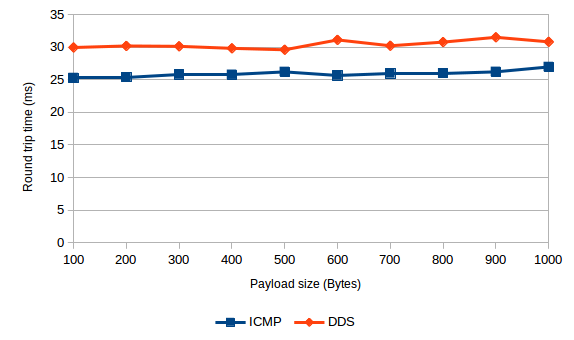
\includegraphics[width=0.7\textwidth]{figures/dds-latency}
  \caption[DDS latency benchmark results]{The average RTT of differently sized packets when using DDS versus ICMP}\label{fig:dds-latency}
\end{figure}

%
%
%
%
%
%
%
%
%
%


\subsection{Failover Test}\label{sec:failovertest}

\paragraph{Motivation.} The presented approach facilitates a wide range of innovative opportunities. For instance, consider the following scenario: A service running on an on-board computer within a vehicle suddenly fails, \eg\ due to a hardware defect. As a reaction, a fallback service needs to take over. Consider now that the fallback service is not running on another on-board computer but within the cloud. Enabled by DDS' failover qualities, the approach allows for a quick switch to the remote backup service. An interesting question is how long the whole failover process, \ie\ switching to a backup service in case of failure, takes in a cloud scenario.


\newcommand{\proda}{\texttt{S\textsubscript{main}}}
\newcommand{\prodb}{\texttt{S\textsubscript{backup}}}
\newcommand{\cons}{\texttt{S\textsubscript{consume}}}

\paragraph{Methodology.}\todo{reference failover mechanism described in previous chapter} To test the performance of DDS's failover qualities an experiment was designed to replicate a scenario in which a service fails so that another, remote service must take over operation. There are three services: two services which continuously produce data (\proda , \prodb) and one which consumes the data (\cons). \proda\ has precedence over \prodb\ (\ie\ it possesses a higher \ownership\ value) and is therefore the "main supplier", while \prodb\ is considered the "backup supplier". 

In the process of sending data, a failure of \proda\ is simulated by abruptly shutting down the application process. Once that happens, a procedure in \cons\ is triggered to determine the time span between the reception of the last message sent by \proda\ and the first message by \prodb . The resulting time is the effective gap between the reception of two messages: the last one from \proda\ and the first one from \prodb . In particular, the measured time includes
\begin{itemize}
  \item the time DDS needs to detect \proda 's change of liveliness and to propagate the change in the system
  \item the time it takes \prodb\ to take over
  \item the transmission time of \prodb 's first message to \cons
\end{itemize} 

\proda\ and \cons\ are deployed as individual applications on two of the Raspberry Pis. \prodb\ is deployed on the remote host. All communication goes through an encrypted Weave network spanning over the LAN and the cloud.

\todo[inline]{which QoS settings were used? how many test runs were conducted? Describe how clocks are synchronized between the two producing services}


\paragraph{Results.} Reliability can be ensured, even when offloading work into a remote data center.

%
%
%
%
%
%
%
%
%
%

\section{Case Study}

\paragraph{Motivation.} Motivation

%
%
%
%
%
%
%
%
%
%



\chapter{Discussion}\label{chapter:discussion}
In \autoref{chapter:approach}, the thesis' main approach was introduced. As part of this, an exemplary technology stack to realize the system was proposed (\cf \autoref{chapter:realization}). The exemplary solution, which is based on DDS, \docker , and \wnet , was then assessed with the aid of a number of benchmarks (\cf \autoref{chapter:evaluation}). In this chapter, the proposed solution is discussed, and its merits as well as its flaws are pointed out. The list of requirements given in \autoref{sec:requirements} and the benchmark results from the previous chapter serve as the foundation of the discussion. 


\section{Requirement Analysis}

\paragraph{Availability/Reliability.}
Moving vehicles are are very likely to lose reception during operation, \eg , when navigating through remote areas. At the center of the presented approach is cloud connectivity, and hence, the reliability of the network is a major concern. Thus, a primary objective when designing the system was to make it as resilient to connection losses as possible. A prerequisite for handling reliability issues is fast failure detection and a quick fail-over mechanism so that timing requirements can be met and downtime is kept at a minimum. With its support for redundancy and failure detection, DDS is perfectly equipped for such cases. DDS' way of guaranteeing reliable information exchange is achieved by QoS policies. For failure detection, DDS employs a liveliness mechanism whereby services are either proactively, or reactively, probed for responsiveness. If a service fails to meet the demand, it is declared ``dead''. In such cases, fallback services may be elected as (temporary) replacement. As soon as the original service's operability restored, it may take over again. Thus, DDS provides a level of reliability that allows the system to handle (intermittent) connection losses and other failures quickly.

While \wnet\ doesn't quite reach the level of replication- and failure transparency provided by DDS, it has other ways to deal with unreliable underlay networks. When a link between two nodes is interrupted \weave\ takes no proactive measures to find an alternative link but it reconnects as soon as connectivity is restored. Thus, a moderate resilience to connection loss is discernible.

\paragraph{Security.}
Security was a major concern when designing the approach. In fact, \weave 's security features were one of the primary reasons why it was chosen as overlay networking technology. In particular, its support for end-to-end encryption ensures the confidentiality and integrity of the communication channel, even in insecure networks such as the Internet. \wnet 's security is based on IPSec and state-of-the-art encryption algorithms. However, questions remain about the usability of \weave 's encryption mechanism. \weave\ employs a shared secret approach, \ie , a password needs to be present on all participating hosts. How this secret is to be securely stored and how situations of leakage are dealt with are an open question yet to be answered.

Aside from encryption, isolation is an important means to improve the security of a system. By integrating isolation measures, security perimeters can be created which are difficult to penetrate. The more layers of isolation there are the better the system can be protected from attackers. The approach leverages \docker\ to provide isolation. Each service instance is running within the perimeters of a container. However, whether \docker 's isolation properties are sufficient in terms of security is debatable \cite{xavier2013performance}. The fact of the matter is, however, that any degree of isolation is better than no isolation. Hence, for now, the security of \docker\ is considered sufficient, although a rigor security analysis is still to be done.

Another aspect that determines a system's level of security is how well it can be updated. Modern systems, and especially those building on high-level OSes, need to be supplied with security updates on a regular basis. \docker 's layered images greatly facilitate software updates as single layers may be swapped out individually. Whenever a new update is to be rolled out only the layer that changed needs to be replaced, and only that one, single layer needs to be downloaded from the server. Thus, \docker\ greatly eases the software update process.


\paragraph{Interoperability.}
The approach is based on containerization as means to achieve a maximum of interoperability. In fact, interoperability is one of its main selling points. \docker\ is used as containerization technology, which allows software to run on any platform that possesses a container engine and has a kernel---properties that is not hard to come by. \docker\ currently supports x86 and ARM. The latter is important to guarantee binary compatibility in embedded systems, which are often based on ARM architectures. Additionally, in recent years, efforts to standardize and unify container technologies were launched. Driven by the \emph{Open Container Initiative}\footnote{\url{www.opencontainers.org}} (OCI), standards aimed at providing interoperability between containerization technologies were created. Thus, interoperability, at least in terms of containerization, is not impaired.

\weave\ is, in its entirety, centered around \docker , and even the \weave\ software itself runs exclusively within \docker\ containers. As a consequence, and unsurprisingly, it may run on any platform which is capable of running \docker\ containers. Thus, hardware interoperability is given. However, due to its dependency to \docker , a lock-in situation is evident. Consequently, in order to swap \docker\ with a competing containerization tool, one would have to drop \wnet\ from the approach. Similarly, when deciding to go without any sort of containerization, \weave\ could not be used anymore.

Apart from this, the chosen messaging middleware, DDS, offers decent interoperability support. The approach suggests to define service contracts by means of topics, and in particular, the combination of their associated name, message data type, and QoS policies. The type is specified in a language-independent format (IDL), and is not bound to a specific technology. Thus, platform-independent service contracts may be realized. Beyond that, DDS also supports platform-neutral communication with its wire protocol, RTPS. RTPS ensures that applications using different DDS implementations may communicate with each other, thereby ensuring a great deal of interoperability and preventing vendor lock-in.

\paragraph{Performance.}
One of the main motivations behind the approach is to support the resource-constrained on-board computing system of vehicles by offloading computations to the cloud, and thereby improve the performance of the whole system. The benchmarks in \autoref{chapter:evaluation} demonstrate that the approach manages to fulfill the performance requirement to a satisfying degree. This is because the employed technologies were chosen, in part, on the basis of their performance properties.

DDS exhibits great performance characteristics because it is, from the ground up, designed to perform well. The fact that DDS employs multithreading-based asynchronous programming, and that virtually all DDS implementations are implemented in C++, underline this statement. In section \ref{sec:ddslatency} DDS was evaluated regarding its latency characteristics in an overlay setting. The results of the benchmark show that DDS incurs reasonable protocol overhead. In that benchmark, DDS was compared to ICMP---a protocol which is not designed for information exchange. The comparison is therefore imbalanced to the detriment of DDS. The fact that DDS still performed comparatively well is a strong argument for its aptitude. 

Similar to DDS, \docker\ was built with performance in mind. Many benchmarks have been conducted which support this statement (\eg\ \cite{adufu2015container, felter2015updated, morabito2015hypervisors, xavier2013performance}). At the same time, \docker\ is very efficient in terms of energy consumption \cite{morabito2015power}. Virtually all performance analyses agree that \docker\ incurs minimal computational and I/O overhead, provided that it is configured properly. One reason why \docker\ performs well is that programs running within containers are actual processes which run directly on the host system's kernel. Thus, no computational overhead is incurred. This is in contrast to VM-based virtualization in which programs run on an intermediate hypervisor layer which affects performance negatively. Furthermore, containers do not have to boot into an operating system, as VMs do. As a result, containers may be launched in a matter of milliseconds.

A slightly less optimistic picture paint the benchmark results for the evaluation of \wnet . The results reveal that the overlay technology adds a barely noticeable latency overhead, even when applying encryption (\cf section \ref{sec:plainlatency}). Likewise, network throughput takes only a minor hit (\cf section \ref{sec:throughput}). However, these properties only apply when enough computing resources are present. In cases where computing power is insufficient, severe network performance degradations may be the result. The reason for this is that overlay networking, \ie\ the wrapping and unwrapping of encapsulated data, puts significant load on the CPU. In section \ref{sec:utilization}, a case was explored in which the test nodes reached their computational limit such that the CPU became the bottleneck. As a result, only a fraction of the theoretically achievable network bandwidth could be utilized. Expressed in figures, the effective throughput stalled at around 23 Mbit/s. The severe computational overhead can be explained by \weave 's custom encapsulation protocol (``sleeve''), which is automatically used for overlays that span over the Internet. In this mode, packets need to traverse the \weave\ router. Because the router is a user space process, many context switches need to be performed during continuous data transmissions. This circumstance causes significant delays if many packets need to be sent in rapid succession. All in all, one can conclude that \wnet\ is definitely not the best suited technology for the use case at hand.


\paragraph{Scalability.}
\todo[inline]{FERTIG MACHEN}
Scalability has been one of the main objectives when designing the system.
system is designed to scale out: 
Services can be replicated in the cloud
new functionality can be easily added through DCPS
Docker promotes statelessness -> no shared state -> easier to scale
Beyond sheer scalability the system has the potential for great \emph{elastic} scaling

\begin{itemize}
\item anonymous multicast communication facilitates scalability. new services don't need to explicitly register to related services. All communication goes to a multicast address. The underlying infrastructure takes care that messages are distributed accordingly.
\item automatic service discovery: it's easy to add new services. It's enough to start the program and the publisher/subscriber can automatically participate in a topic.
\item Decentralization also improves scalability: In centralized systems, there is often a single point of failure which may be overloaded with increasing demand. 
\item However, performance properties when adding publishers or subscribers was not tested. Previous work?
\end{itemize}

With \docker\ it is easy to replicate services. 
\begin{itemize}
\item \docker\ can be controlled via mature RESTful API which makes it easy to launch containers in a unified manner
\item Container spin-up is extraordinarily fast. Helps elasticity.
\end{itemize}

Adding containers to a \weave\ overlay happens implicitly when the host is already running a \weave\ router. Starting the \weave\ router on a machine can be done at system start up via shell script. Gripe: It is not known if \weave 's performance degrades with many nodes in the overlay. This is future work.

(Weave nodes can be easily integrated into existing networks. When the \weave\ router is already in place on a host, merely starting a container is enough to connect it to the overlay.)

\paragraph{Extensibility.}
The extensibility of the approach is to a large extent facilitated by DDS, and in particular, the publish-subscribe paradigm. In the DCPS paradigm, data is provided ``as is'', \ie , there are no implications or restrictions \wrt\ how that data is used. A newly added service is not concerned with the original \emph{purpose}, or intent, of the data, nor can any other service dictate how the data is supposed to be used---a service just takes advantage of the \emph{presence} the data. Hence, data can be reused in ways that weren't even intended when first designing the system. By having no connotations about the data's semantics, new services can be easily added without making changes to a service's interface, or affecting other parts of the system. Extensibility is further improved by DDS's dynamic service discovery. A newly added service can subscribe to any topic at run-time, as long as the topic's name and type are known. Similarly, a service which provides data may register new topics at will and can engage in collaboration instantaneously. At the same time, other services are entirely oblivious to the fact that a service was added. The change of topology is handled exclusively by the middleware, and minimal manual effort is needed to integrate new services.

\wnet\ also helps in building extensible systems: software as well as hardware nodes can be easily added to existing overlays. \weave\ overlays are set up at host-level, \ie , each host participating in an overlay has the \weave\ daemon running on it. The daemon causes any container that is launched on such host to be automatically added to the overlay. There is no need for per-container configurations or scripts to be executed, which significantly eases the way software nodes may be added to the system. This process is entirely transparent, so that a container management and orchestration system does not even have to know that \weave\ is in place. \weave 's extensibility properties also carry over to the hardware-level. If a new hardware node were to be added to the system, the only thing one would have to do is launch the \weave\ software on that node, referencing the IP address of at least one other participating node. The other node would then propagate the addition of new node in the whole overlay. Shortly after, every other node in the system would know that a new node was added. This self-governing approach minimizes manual work, and thus, benefits extensibility greatly.

To further improve the system's run-time extensibility it must facilitate software updates. How \docker\ aids in realizing efficient software updates has already been discussed.


\paragraph{Adaptability.}
A major challenge in automotive systems is run-time adaptability. Due to their dynamic nature, vehicles are exposed to rapidly changing situations which require quick and adequate reactions. An example of a situation that needs to be handled quickly is a hardware failure. The approach utilizes DDS' failover mechanism to handle such situations. An example of this was demonstrated in section \ref{sec:failovertest}. The same principle can be applied when the vehicle is succumbed to intermittent connectivity: when the vehicle loses reception while using a cloud-based service, the system can quickly switch to a vehicle-based service. Potential for more advanced ways to deal with operational situations is provided by \docker . The \docker\ daemon exposes an API by which containers can be started and destroyed remotely. One could think of a central management and orchestration component which monitors the state of the system and, with help of the API, can start and stop services, depending on situational demand. 

Other aspects of adaptability are the ability to react to changes in requirements by means of software updates, and adaptability in terms of platform independence. Both aspects have already been discussed.


\paragraph{Testability.}
With the help of containers, software can be made portable so that it can run on a variety of platforms. This principle is taken advantage of by CI/CD platforms. CI/CD pipelines, in general, perform the following steps: first, the application's program code is downloaded from its source code repository to dedicated CI servers whenever changes are committed to the repository. Then, the software is built and all automated tests are run. In this step, containers are often used  \cite{barna2017delivering} to guarantee the processes' determinism: building and testing the software within containers ensures that all dependencies are available and that the result of successive builds is always the same. Consequently, the built program runs on the developer's workstation, the CI server, and the production server in the exact same way.
When one of the tests fail, the development team is notified instantaneously so that they can fix the error as soon as possible. If all tests pass, the software is automatically deployed to the production environment. This process ensures rapid development velocity, and more importantly, helps to verify the correctness of the software during the whole development cycle. This principle was demonstrated in section \ref{sec:multiplat}, were a minimal CI/CD pipeline was described. Although the presented pipeline did not include an automated testing step, such step could be easily integrated. 

%
%
%
%
%
%
%
%
%
%
\section{Limitations}
The benchmarks in the previous chapter demonstrated that the approach to cloud connectivity presented in this thesis is fully functional and performs reasonably well. However, the prototypical implementation is far from perfect and comes with a number of limitations that need to be addressed.

As the presented implementation is merely a proof of concept, several aspects were insufficiently evaluated. First and foremost, little attention has been paid to the safety requirements of vehicles. \wnet\ is not designed to be used in safety-critical systems. On their website, Weaveworks make no statement about any certification efforts that make the software suitable for the use in safety-critical scenarios. Thus, for the time being, the presented approach may only find applicability for non-safety critical functions, \eg\ in the context infotainment systems. However, it may be added that \wnet\ is open source, and as such, all underlying technologies and concepts are disclosed. Thus, it is entirely possible to implement a thoroughly verified and tested derivative of \wnet\ tailored to safety-critical systems.
The same is true for \docker . \docker\ just so happens to be the most mature containerization technology, which is why it was chosen for the prototype. However, \docker\ is by no means suitable for safety-critical systems. But like \wnet\ , the concepts that underly \docker\ are based on well-known technologies and it is entirely transparent how \docker\ works under the hood. Furthermore, it may be noted that the \docker\ images presented in this thesis are not meant to be used in production. Although there was an effort to minimize the size of the images, in real scenarios, images would be shaved down to the bare minimum, both in terms of size and capabilities. Utilities such as compilers, build tools and generally everything which is not a prerequisite to execute a given service would be removed. The images used in this thesis serve the purpose of demonstration and thus, such measures were not taken to ensure a rapid progression of this work. More time would be needed to optimize the images for production use. Additionally, more measures are required to improve the containers' isolation. For example, the number of system calls that a containerized process can invoke should be reduced significantly through tools like \emph{SELinux}.

Another limitation related to the used technologies is that they are not universally usable on all hardware platforms. For example, \docker\ requires the substrate system to run a Linux kernel and a container runtime. This requirement is hard to fulfill in many cases, \eg , for the use with smart phones. This circumstance further restricts the system's potential use cases.

An additional aspect which was negligently evaluated is security. Although \linebreak\wnet\ promises to provide end-to-end encryption, it is unknown how effective and robust the employed encryption scheme is. A rigor security analysis is needed to be able to make a well-founded statement about this aspect. Furthermore, questions about the encryption mechanism's usability remain unanswered. To encrypt a \weave\ overlay, all hardware nodes need to be supplied a shared secret. The question how this secret shall be distributed and stored securely was not answered in this thesis. 
Another major caveat concerning \weave 's usability is its extensive resource utilization.  When overlays span over long distances, \weave\ employs a custom encapsulation protocol which is applied by a user space process. Thus, a context switch is needed for every packet that is sent, making this process highly inefficient. This circumstance was demonstrated in section \ref{sec:utilization}, where the effect of overlay networking on CPU utilization was investigated. The results of this experiment show that \weave\ overlays may introduce CPU-bound bottlenecks for high-throughput applications. As energy efficiency is one of the main motivating factors behind the devised system, one can conclude that \wnet\ is unsuitable in automotive use cases.

Overall, the provided implementation is not, in any way, suitable for production use in vehicular environments. This, however, was never the goal of this thesis. \wnet\ and \docker\ were both chosen for the lack of better alternatives. Furthermore, both tools provide easy-to-use interfaces which allowed for quick prototyping, ensuring the rapid progression of this thesis. 


\chapter{Related Work}\label{chapter:related-work}
Cloud computing in the context of automotive allows for the realization of disruptive innovations which have great potential to improve driver satisfaction and to open up new fields of business for car manufacturers. For instance, \citeauthor*{wollaeger2012cloud} propose a framework which allows for the computation of an optimal velocity profile for vehicles in an effort to minimize fuel consumption \cite{wollaeger2012cloud}. Their solution benefits greatly from the vast amounts of computing resources available to clouds as it relies on dynamic programming which is characterized by high resource demands. Furthermore, large amounts of data are accessible in the cloud which may be used to make better-informed decisions, \eg\ on the basis of crowd-sourced data pools.

While some approaches exist which explore possible use cases of automotive clouds, very little work can be found that addresses the \emph{architectural} challenges of creating cloud-supported systems specifically for the automotive domain.
Thus, much of the work related to this thesis is concerned with other, more researched domains, such as IoT and fog computing. First and foremost, the thoroughly executed and exhaustive survey on fog computing \cite{nath2018survey} by \citeauthor*{nath2018survey} shall be mentioned as highly relevant and recommended reading. In their literature study, the authors present and summarize work pertaining to a variety of subjects related to IoT and embedded computing.
An important and much-discussed aspect in this domain is the \emph{management} of the of widely dispersed collections of embedded computing nodes that make up pervasive IoT systems. Similar to the system proposed in this thesis, many approaches exist that attempt to master the complexity inherent to these systems by means of service-oriented computing. Notable examples of service-oriented architecture frameworks tailored specifically to the IoT and CPS are the SOCRADES project \cite{cannata2008socrades}, the IMC-AESOP project \cite{karnouskos2012soa} and the ARUM project~\cite{marin2013conceptual}.
Further noteworthy approaches are presented in \cite{butzin2016microservices}, \cite{kart2007distributed}, and~\cite{teixeira2011service}. 
A common denominator among these works is the idea to represent heterogeneous physical resources and processes as software objects that can be managed and controlled programmatically and may interact with each other by means of machine-to-machine interfaces.
Of particular interest for this thesis are furthermore service-oriented approaches specifically tailored to \emph{automotive} systems. Contributions in this domain are provided, \eg , by \citeauthor*{kugele2017service}. In their paper \cite{kugele2017service}, the authors present the results of an interview study investigating the needs of automotive software architects and conclude that SOA-based approaches to E/E-system modeling bring promising benefits to the automotive development process. A concrete example of how service oriented modeling can have great benefits for the development of ADAS is presented by \citeauthor*{wagner2014developing} \cite{wagner2014developing}. 


%\paragraph{Embedded SOA}
%\begin{itemize}
%\item \cite {scholz2009soa}: \citeauthor*{scholz2009soa} - ∈ SOA-Service Oriented Architectures adapted for embedded networks
%\item \cite{wagner2014developing}: \citeauthor*{wagner2014developing} - Developing self-adaptive automotive systems - On the integration of service-orientation into automotivedevelopment processes -- SOMA4DDAS
%\end{itemize}

Most of these architectural approaches stay in the local domain and do not consider cloud connectivity. A common method to bridge the gap between local computing clusters and remote data centers is to employ middlewares.
\citeauthor*{farahzadi2017middleware} analyze the problem domain of cloud connectivity for the IoT (``Cloud of Things'')\cite{farahzadi2017middleware}. For this purpose, they present a survey in which they analyze a number of different IoT middleware solutions and compile a set of key challenges and requirements for such systems. They furthermore introduce a taxonomy to group types of middlewares and map each of the 20 investigated middlewares to one of the groups. 
Particularly interesting are middlewares that, similar to this thesis' approach, focus on publish-subscribe-style communication.
For instance, \citeauthor*{antonic2016mobile} present COPUS~\cite{antonic2016mobile}, a cloud-based publish-subscribe middleware for the IoT. In the paper, the authors perform benchmarks to evaluate the middleware with respect to scalability and elasticity and present a case study in which test subjects were equipped with mobile air quality monitoring sensors that would continuously send sensor data to the cloud. COPUS relies on a broker as cloud gateway which must be installed on a mobile device (\eg\ a smartphone). Thus, this solution is unsuitable for the automotive domain.
Further noteworthy publish-subscribe middlewares for the IoT are HoPP \cite{gundougan2018hopp} and VIRTUS \cite{bazzani2012enabling}.

Publish-subscribe enables anonymous point-to-multipoint communication which brings universal benefits, such as scalability and extensibility, which are also interesting for the automotive domain.
Thus, several projects exist that aim to implement publish-subscribe in vehicular E/E architectures.
An example for this is the RACE project \cite{sommer2013race}, an effort to create a holistic platform for next generation cars.
An industry-driven project with the same goal is the AUTOSAR Adaptive Platform \cite{furst2016autosar}.
Noteworthy in this regard is also SOME/IP \cite{volker2013some}, an IP-based automotive middleware by which vehicular functions can be modeled in a service-oriented fashion. SOME/IP integrates flawlessly into AUTOSAR and supports publish-subscribe and other communication paradigms.

The exemplary implementation presented in this thesis relies on the DDS middleware for data exchange. Unfortunately, at the time of this writing, only few attempts were made that aim to leverage DDS in the context of vehicles (\eg\ \cite{bouhouch2013dds, bouhouch2011implementation}). However, some work was done that is concerned with the use of DDS in other safety-critical systems. \citeauthor*{perez2017handling}, for instance, explore DDS for ARINC-653-based avionic systems~\cite{perez2017handling}.
The same authors furthermore present a way to combine DDS and hypervisor-based inter-process communication to interconnect a time and space partitioned system \cite{perez:gutierrez:ieeetpds16}. Their focus lies on mixed-criticality applications running atop a hypervisor designed for safety-critical scenarios. The performance tests they conduct show that DDS adds a reasonable overhead to the communication performance but the overhead caused by hypervisor-based partitioning is quite significant, albeit reducible by the use of multicore processors.
Significant contributions in this field were also made by \citeauthor*{serrano2013virtualizing}, who investigate the performance impact of virtualization on DDS-based applications~(\cite{serrano2013virtualizing, garcia2013benchmarking}).

DDS in combination with overlay networks is another highly relevant topic for this thesis. Only one contribution was found that investigates this opportunity:
\citeauthor*{hakiri2015publish} devise a system to interconnect IoT devices via DDS over overlay networks \cite{hakiri2015publish}. However, the description of their approach lacks details and no real effort were made to evaluate it.
Another relevant work related to overlay networking is presented by \citeauthor*{kratzke2017microservices}. In his paper \cite{kratzke2017microservices}, the author investigates the performance impact of using encrypted overlay networks (in particular, \wnet ) for Linux containers on top of hypervisors. This setup---containers atop hypervisors---is very common in cloud scenarios as IaaS providers often provision servers in the form of virtual machines. This is also the case for the test setup described in this thesis. The author concludes that containers add a non-negligible impact on networking performance. In \wnet -based overlay networks, the performance is further impaired, and another, less-significant impact is observed when employing encryption. This is in contrast to the benchmark results presented in this thesis, which suggest that both technologies incur a very minor overhead.

\paragraph{}
This thesis' approach relies on containerization as means to encapsulate functionality in isolated, portable units. A challenge in this is to marry containerization with the traditionally resource-constrained embedded systems. In recent years, this prospect has received substantial attention in the research community. For instance, \citeauthor*{morabito2017virtualization} provides an in-depth analysis on the utilization of container technology for a variety of Single-Board Computers \cite{morabito2017virtualization}. The author's evaluation includes benchmarks that assess energy consumption, device temperatures, as well as I/O and computing performance and other factors.
Further analyses and benchmarks are presented in \cite{pahl2015containers} and \cite{bellavista2017feasibility}.  
The evaluations reach a consensus that containerization for resource-constrained devices presents a promising prospect. 
In fact, the industry has already caught on.
resin.io\footnote{\url{www.resin.io}} is a project dedicated to bringing containers to embedded devices. In the past, resin.io have made several significant contributions to enable container-based Continous Integration for embedded systems, and have also taken initiative to further minimize resource requirements of containerization. To this end, resin.io provide their own light-weight container engine called ``balena''\footnote{\url{www.balena.io}} and an accompanying host OS that is deliberately crafted to run containers (``resinOS''\footnote{\url{www.resinos.io}}).


%\paragraph{computation offloading in cloud (cell phones)}
%\citeauthor*{barbera2013offload} \cite{barbera2013offload} analyze in which cases it is sensible to offload computations from cell phones to the cloud. There is a tradeoff to be made between the energy savings achieved by the offloading itself and the increased computational overhead of sending data over a mobile network. They aim to provide virtual replicas of the hardware in the cloud, running at all times alongside the physical device to support it whenever there is a need. They do not consider statelessness of the replicas and employ a synchronization mechanism to keep the state consistent. This incurs additional overhead. They use cell phone specific tools which are inapplicable in the automotive use case. They view their approach as holistic solution -> lack of flexibility

%In \cite{chun2011clonecloud} \citeauthor*{barbera2013offload} present \emph{Clone Cloud}, a system to offload workload from mobile applications to the cloud. They employ a combination of static analysis and dynamic profiling to automatically partition mobile applications. repartitioning is thread-wise. They achieve a 20-fold execution speed-up and 20-fold decrease of energy consumption.

\paragraph{}
Finally, after having covered related work concerning the basic building blocks of this thesis' approach (architecture, communication and virtualization), there are some pieces of related work that use similar methods (combining the aforementioned concepts) to achieve similar goals.

One example is presented by \citeauthor*{berger2017containerized}. In their paper \cite{berger2017containerized}, the authors describe their experiences of employing containerization in the context of self-driving vehicles.
In accordance with the microservice architecture pattern, vehicular functionality in their approach is split into a number of fine-grained services deployed on distributed nodes within the vehicle. The services are connected via OpenDaVINCI, a real-time-capable middleware for distributed embedded systems. This approach is very similar to the one proposed in this thesis in that communication is based on multicast-enabled publish-subscribe and that they employ \docker\ containers. However, their approach lacks cloud connectivity. The authors furthermore struggle to get multicast to work over Docker overlay networks---a problem that was solved in this thesis.
%The interplay of their services is based on a \emph{pipes-and-filters} methodology.
%Multi platform images are achieved through different base layers employing different compilers. Disadvantage: containers cannot be moved freely between nodes of different hardware architectures.
%questionable design decisions: Centralized configuration protocol... but decentralization is key
%Suggest to have private registry within the vehicle.
%To provide a high degree of tracability, they present a versioning system that allows versioning of individual image layers which seamlessly integrates into their development workflow.
%Similarly, \citeauthor*{schneider2016achieving} \cite{schneider2016achieving} use containerization in a microservice environment for vehicular functionality. However, the authors only focus on the backend part, \ie , services provisioned in data centers that vehicles may connect to. Their approach does not consider the use of microservices \emph{within} the vehicle. In addition, their methodology is described in rather vague terms and lacks detail.

Another approach that resembles the one presented in this thesis is described by Asad \citeauthor*{javed2016container}. In his master's thesis \cite{javed2016container}, he explores the possibility of managing IoT nodes via \docker\ containers and the Kubernetes\footnote{\url{www.kubernetes.io}} container orchestration platform. The employed experimental setup is very similar to the one used in this thesis in that a local cluster of Raspberry Pis is connected in a LAN with cloud access. Attached to some of the Raspberry Pis are cameras that capture images which are then sent to the cloud via Apache Kafka. Like in this thesis, communication between the nodes and the cloud is publish-subscribe-based. However, the approach has a serious drawback: Kubernetes and Kafka are technologies designed for sophisticated cloud environments and are by no means suitable for the use within embedded computer networks due to their tremendously high system requirements. Moreover, no serious effort is evident to evaluate the approach in a neutral manner.

\citeauthor*{grossmann2016hypriot} describe another approach \cite{grossmann2016hypriot} related to the previous one. But instead of heavy-weight enterprise container management solutions they follow a more light-weight philosophy. A drawback of their approach is a lack of failure resiliency inherent to their centralized architecture in which a master node may become a single point of failure. A follow-up to that work is presented by \citeauthor*{celesti2017watchdog} in which several weak points are addressed \cite{celesti2017watchdog}.

%The fact that ubiquitous publish-subscribe is not only a research matter but is also the basis of multiple commercial industry products is proof for its value. 
Not only in the research community, but also in the industry, there is interest in ubiquitous publish-subscribe. 
For instance, PubNub\footnote{\url{www.pubnub.com}} is a commercial service that aims to provide publish-subscribe-style communication for large numbers of devices dispersed on a global scale. Their focus lies on IoT devices and mobile phone applications. Thus, there is a pronounced focus on handling mobility challenges such as frequently changing IP addresses and general reliability issues. PubNub is a holistic, all-in-one solution, \ie , their service includes everything from client APIs to infrastructure provisioning. The fact that \mbox{PubNub} is a closed platform severely inhibits its adaptability and limits its applicability---especially for the automotive use case, which is characterized by highly specific requirements. While it may be true that PubNub is a good starting point to kick off new businesses (as advertised), it is doubtful that it is the right tool for the intended use case.

Another commercial product that follows the same goal, but is focused more on Industrial IoT (IIoT), is offered by ADLINK (formerly PrismTech). ADLINK provides a holistic data sharing platform based on DDS named ``Vortex DDS''. Aside from their own DDS implementation, OpenSplice, the Vortex platform includes the service called ``Vortex Cloud''.\footnote{\url{www.prismtech.com/vortex/vortex-cloud}} Like this thesis' approach, Vortex Cloud aims to connect globally dispersed DDS components, and also provides means to deploy DDS-based applications in the cloud. Unfortunately, no information about the inner workings of Vortex Cloud and its aptitude can be found online. As it is a commercial, closed-source product, this option was not further pursued.

Real-Time Innovations (RTI) is another company which provides an DDS implementation called ``RTI Connext DDS''.\footnote{\url{www.rti.com/products}} A salient feature of Connext is that it supports DDS-based data transmission over WANs natively. However, this ``RTI Secure WAN Transport'' has several drawbacks. Firstly, it needs to be configured on code-level in all applications that participate in the communication network. This is in contrast to this thesis' approach in which the applications themselves are kept unaware of the fact that they are communicating with peers outside their LAN. This agnostic approach promotes loose coupling, simplifies network management, and ultimately enables applications to migrate freely between computing nodes. Further disadvantages of RTI's approach are that it doesn't support multicast, that it requires a central ``rendezvous'' server which acts as a participant repository, and that it is not resilient to connection loss.\footnote{\url{community.rti.com/static/documentation/connext-dds/5.3.0/doc/manuals/connext_dds/html_files/RTI_ConnextDDS_CoreLibraries_UsersManual/index.htm}}

%For this, a central, publicly accessible ``Cloud Discovery Service'' is required which acts as a repository that holds all participating applications' locations.



\chapter{Conclusion}\label{chapter:conclusion}
To conclude this thesis, a summary is first given in which the context, problem statement, and the chosen approach is recapitulated. Then, ideas for future research opportunities are provided.

\section{Summary}\label{sec:summary}
\subsection{Context}
Current trends in the field of automotive mobility, such as autonomous driving, are the cause of an increased demand for computational power and the need for advanced data collection techniques. Associated with this development is an inherent increase in energy consumption. However, an objective should be to keep the energy usage of vehicles' electronic systems as low as possible. This applies especially in the wake of the ever-increasing importance of electro mobility where every bit of energy is needed to fuel the vehicle. In the face of this dilemma traditional vehicular on-board technologies are reaching their limits, and thus, new ways to tackle tomorrow's mobility challenges need to be investigated. One possibility to overcome the constraints imposed by the limited capabilities of current vehicles' computing infrastructure is offered by \emph{cloud computing}. Cloud computing has been around for many years now and many modern businesses thrive on the innovation opportunities that cloud technologies facilitate. However, comparatively little attention has been paid to the prospect of integrating them into the automotive domain. A reason for this might be the special requirements that apply to this particular industry. The most prominent challenge is the mobility aspect of vehicles which makes it difficult to maintain a reliable communication channel to the outside world. This issue will be greatly alleviated with the upcoming 5G cellular network that is currently being rolled out. Supported by such technologies, cloud computing paves the way for new, innovative functions for tomorrow's vehicles. For example, computationally intensive tasks could be offloaded to high-performance computing systems with the aim of relieving the vehicle's constrained on-board system, and to boost the system's performance. Further potential lies in the simplified collection of telemetry data for real-time health monitoring and remote troubleshooting as well as in the provisioning of backup services for safety-critical functions.

\subsection{Approach}
This thesis was created as a response to the situation laid out in the previous section. The goal of this work was to present a system that connects vehicles to clouds as means to facilitate innovative applications. For this, an approach was chosen that lends many concepts from classic bus systems in which dispersed components communicate with each other anonymously by reading and writing messages to a shared, logical medium. The characteristic that makes the approach special is that this medium is virtually extended into the cloud with the help of network virtualization. As a result of this, everything that is put onto the bus can be read from within the cloud. Similarly, applications in the cloud can push data onto the bus, which can then be consumed by the vehicle's on-board system. The approach employs anonymous multicast communication in order to provide location transparency: in the eyes of the vehicle it does not matter whether a given data sample originated in the vehicle or anywhere else. This greatly facilitates the offloading of vehicular functionality into the cloud. The approach builds on a service-oriented architectural paradigm in which the vehicle's functionality is split into a discrete number of \emph{services}. Each service fulfills a purpose which, in traditional E/E architectures, would correspond to an ECU's functionality.

Three key challenges were identified that need to be tackled in order to realize such system. Firstly, reliable, anonymous information exchange needs to be facilitated such that individual services are able to communicate in a reliable manner, without the need for explicit references to one another. For this purpose, DDS was proposed. DDS, being a messaging middleware designed for mission- and business critical systems with high reliability and real-time requirements, is a perfect match for the automotive use case.
%is an open messaging middleware standard for distributed applications. The standard is designed for mission- and business critical systems with real-time requirements. As such, it is a perfect match for the automotive use case. 
The foundation of these properties is laid by \emph{QoS policies}, which serve to control the level of reliability and to establish interface contracts between services. For data dissemination, DDS employs the data-centric publish-subscribe communication paradigm by which data is made available through \emph{topics}. Contrary to RPC-style communication, in which data exchange is based on \emph{instructions}, DDS places \emph{data} at center-stage. Any service that wishes to expose a certain kind of data may \emph{publish} respective data samples on a topic associated with that data. Conversely, any service that is interested in the reception of that sort of data may \emph{subscribe} to that topic. Communication takes place entirely anonymously, \ie, services do not know their peers, and consequently, can not address each other directly. The subsequent dissemination of data is then performed by the DDS middleware ``under the hood''. This approach to information exchange greatly facilitates scalability and extensibility.

In order to enable services to run on both, the vehicle and the cloud, they need to be portable, which poses the second challenge to be tackled: isolation. The approach intends services to be packed into self-contained execution environments with all their dependencies. This would allow them to run independently from each other, on a variety of platforms. To achieve this, the use of containerization technology, and in particular, \docker , is proposed. Containers provide OS-level isolation through kernel namespaces. Namespaces wrap a set of system resources and present them to the container process as if they were dedicated to it. Each aspect of a container runs in its own namespace and its access is limited to that namespace. Similarly, containers have by default no access to the host's filesystem. Instead, they come with their own ``cutout'' of a filesystem which is specified in each container's respective image. In that image, all of a containerized application's dependencies and its runtime are contained. Containers thus provide portability across a multitude of operating systems. The only prerequisite is that the host OS runs on a kernel and provides a container runtime. What makes containers especially appealing for the intended use case is that they exhibit excellent performance attributes, that they may be launched in a matter of milliseconds, and that they may be controlled via HTTP API. The latter characteristic makes it possible to programmatically launch and tear down individual containers in a uniform manner, establishing the basis for orchestration tools like Kubernetes and elasticity controllers.

The last remaining challenge to realize the system is to connect the dispersed services with each other in a location transparent manner. As means to achieve this, SDN-assisted overlay networks were suggested. To demonstrate the general feasibility of the approach, \wnet\ was selected for this purpose. \wnet\ is a tool which aims to enable advanced overlay networking capabilities for \docker\ containers which are dispersed throughout different cloud environments. \docker\ itself comes with intrinsic overlay networking out of the box, however, encryption and multicast is not supported, which is a crucial requirement for the intended use case. \weave\ is implemented as a daemon that runs on all hosts that participate in the overlay. Whenever a container is launched on such host, the daemon automatically adds the container to the overlay. Changes in the topology are constantly propagated to other containers via spanning tree-based broadcast and a gossiping protocol. \weave\ effectively creates a self-governing service mesh in which nodes communicate through VXLAN tunnels. In this mesh, containers may communicate freely with each other across physical boundaries. From the viewpoint of a container it does not matter whether a communication partner is located on the same host or on a remote server in a data center. 

\paragraph{}
The three technologies described above (DDS, \docker , and \wnet ) were combined in a novel way to realize an exemplary implementation of the envisaged system. Selected aspects of this setup were evaluated in \autoref{chapter:evaluation}. In that chapter, a number of benchmarks were presented which serve to demonstrate the approaches' general feasibility and to evaluate its performance attributes and fail-over characteristics. The results of the benchmarks prove that the approach, in itself, performs extraordinarily well. Network latency as well as throughput take only a minor hit in \weave -enabled overlays. Similarly, DDS adds a moderate, but justifiable, overhead. However, severe deficiencies were discovered in \weave 's overlay implementation as it puts a tremendous load on CPUs. The (admittedly feeble) test nodes hit a CPU-bound wall quite early in the throughput benchmark, effectively prohibiting high-volume data transmissions. Especially in consideration of the goal to reduce energy consumption, this insight leads to believe that \wnet\ is not the right tool for the job. Nevertheless, the general feasibility of using VXLAN-based overlays and DDS as means to connect widely dispersed containers was demonstrated successfully.

\section{Future Work}
Although considerable effort was made to quantify the quality attributes of the approach, it is far from being fully evaluated. Future research could investigate many questions which were left unanswered in this thesis. Especially \wnet , which is a technology rooted in the software industry, and has no bonds to the scientific domain, would greatly benefit from further research efforts. Questions of interest would be, for example: To which extent can \wnet\ scale to a greater number of nodes, and does it suffer from performance degradations with an increase in participating entities? How fast can \wnet\ adapt to changes in the underlay's topology? Can it deal with nodes getting assigned new IP addresses? It was furthermore stated that nodes in a \wnet\ overlay automatically reconnect when they lose connection to the other nodes---how fast can the reconnection be accomplished? To which degree does \weave 's sleeve mode impact performance, compared to fast datapath mode? Can \weave\ be used in elastically scaling PaaS systems or Amazon's EC2? Apart from all that, how does \weave\ compare to other, competing technologies, such as \emph{flannel}\footnote{\url{www.github.com/coreos/flannel}} and \docker 's native overlays?

These questions assume that it is worth pursuing \wnet\ as overlay networking technology. This, however, in itself is an unanswered question. Because, as it stands, \wnet\ is the major weak point of the approach. While it is still the only viable solution available, as it supports encryption and IP multicast, many deficiencies relevant to the automotive use case are evident. However, the underlying principles are well known and well understood, and the general feasibility of the these principles was successfully demonstrated in this work. Thus, there are no technical barriers to realizing a system based on the underlying concepts which is better suited for the automotive use case. 

A weak point in the testing methodology which pervades throughout all benchmarks in \autoref{chapter:evaluation} is that the tests were performed under laboratory conditions. The setup was connected to the cloud by means of a stable broadband Internet connection. These conditions obviously don't apply to real life scenarios. Thus, further testing in such scenarios would be required to make a grounded assessment of the approaches' real-world applicability. Optimally, the system would be integrated into a real, moving vehicle with 5G-enabled Internet access. In this context, it would also be interesting to see to which extent the approach would benefit from 5G's rich set of innovative features, such as \emph{network slicing}---a novel way to facilitate advanced network scaling techniques. By means of slicing, the network is separated into a number isolated slices which are then used by different applications. Each slice is highly specific to its application's use case and can enforce corresponding QoS requirements\todo{citation}. Intuitively, the approach, and especially systems based on DDS, would benefit greatly from this. However, further tests would be required to investigate this possibility.

Further research potential lies in the continuing exploration of farther-reaching use cases. This work investigated only a small subset of possible applications facilitated by publish-subscribe communication in overlay networks. A major strength of the approach lies in its ubiquity, \ie\ it is meant to be applied in systems consisting of many interconnected entities. So far, however, only the ``vehicular cloud'' use case was investigated. While a vehicle, with all its contained ECUs, is in itself a distributed system, only dozens of components are connected. It would be interesting to see the approach being used in other use cases in which not dozens, but thousands, of entities are present, \eg\ in the context of sensor networks and other (industrial) IoT applications. 
%Another possible use case would be an V2X scenario in which not a single vehicle is connected to the cloud, but also vehicles among each other.

An aspect that was neglected in this thesis is the management and orchestration of nodes. This thesis only presents the technical foundation to create a system to distribute computational workloads. A possible next step would be to create a central management component which controls the placement of services, similar to container orchestration systems like Kubernetes or Docker Swarm. Using \docker 's programmatic API, containers can be created and destroyed remotely, allowing containers to migrate between different computing nodes. The management component could determine the optimal placement of each service and then use \docker 's API to change each service's location dynamically, according to demand. In case of a temporary peak in computational load, the management component could launch additional service instances in the cloud, leveraging horizontal scaling mechanisms. A first step in this direction was already taken with a research paper that was composed to investigate this very prospect \cite{kugele:hettler:itsc}.


%% !TeX root = ../main.tex
% Add the above to each chapter to make compiling the PDF easier in some editors.

\chapter{Test}\label{chapter:test}

\section{Section}
Citation test~\parencite{latex}.

\subsection{Subsection}

See~\autoref{tab:sample}, \autoref{fig:sample-drawing}, \autoref{fig:sample-plot}, \autoref{fig:sample-listing}.

\begin{table}[htpb]
  \caption[Example table]{An example for a simple table.}\label{tab:sample}
  \centering
  \begin{tabular}{l l l l}
    \toprule
      A & B & C & D \\
    \midrule
      1 & 2 & 1 & 2 \\
      2 & 3 & 2 & 3 \\
    \bottomrule
  \end{tabular}
\end{table}

\begin{figure}[htpb]
  \centering
  % This should probably go into a file in figures/
  \begin{tikzpicture}[node distance=3cm]
    \node (R0) {$R_1$};
    \node (R1) [right of=R0] {$R_2$};
    \node (R2) [below of=R1] {$R_4$};
    \node (R3) [below of=R0] {$R_3$};
    \node (R4) [right of=R1] {$R_5$};

    \path[every node]
      (R0) edge (R1)
      (R0) edge (R3)
      (R3) edge (R2)
      (R2) edge (R1)
      (R1) edge (R4);
  \end{tikzpicture}
  \caption[Example drawing]{An example for a simple drawing.}\label{fig:sample-drawing}
\end{figure}

\begin{figure}[htpb]
  \centering

  \pgfplotstableset{col sep=&, row sep=\\}
  % This should probably go into a file in data/
  \pgfplotstableread{
    a & b    \\
    1 & 1000 \\
    2 & 1500 \\
    3 & 1600 \\
  }\exampleA
  \pgfplotstableread{
    a & b    \\
    1 & 1200 \\
    2 & 800 \\
    3 & 1400 \\
  }\exampleB
  % This should probably go into a file in figures/
  \begin{tikzpicture}
    \begin{axis}[
        ymin=0,
        legend style={legend pos=south east},
        grid,
        thick,
        ylabel=Y,
        xlabel=X
      ]
      \addplot table[x=a, y=b]{\exampleA};
      \addlegendentry{Example A};
      \addplot table[x=a, y=b]{\exampleB};
      \addlegendentry{Example B};
    \end{axis}
  \end{tikzpicture}
  \caption[Example plot]{An example for a simple plot.}\label{fig:sample-plot}
\end{figure}

\begin{figure}[htpb]
  \centering
  \begin{tabular}{c}
  \begin{lstlisting}[language=SQL]
    SELECT * FROM tbl WHERE tbl.str = "str"
  \end{lstlisting}
  \end{tabular}
  \caption[Example listing]{An example for a source code listing.}\label{fig:sample-listing}
\end{figure}


\appendix{}

\microtypesetup{protrusion=false}
\listoffigures{}
\listoftables{}
\lstlistoflistings{}
\microtypesetup{protrusion=true}
\printbibliography{}

\end{document}
